\documentclass
[
  draft    = true,
  fontsize = 11pt,
  parskip  = half,
  BCOR     = 0pt,
  DIV      = calc,
  ngerman,
  usenames,
  dvipsnames
]
{scrartcl}

\usepackage[utf8]{inputenc}
\usepackage[T1]{fontenc}
\usepackage{lmodern}
\usepackage{babel}
\usepackage{amsmath}
\usepackage{amssymb}
\usepackage{tikz}
\usepackage{xcolor}
\usepackage{siunitx}

% Das Zeichen := in einer zentrierten Version
\mathchardef\ordinarycolon\mathcode`\:
\mathcode`\:=\string"8000
\begingroup \catcode`\:=\active
  \gdef:{\mathrel{\mathop\ordinarycolon}}
\endgroup

\pagestyle{empty}

% ------------------------------------------------------------------------------
\begin{document}
% ------------------------------------------------------------------------------

% height of a fraction in displaystyle
\newsavebox{\dummy}%
\sbox{\dummy}{$\displaystyle\frac{b}{a}$}%
\newlength{\ruled}%
\setlength{\ruled}{\dp\dummy}%
\newlength{\rulet}%
\setlength{\rulet}{\ruled}%
\addtolength{\rulet}{\ht\dummy}%
\newcommand{\colgap}{\rule[-\ruled]{0pt}{\rulet}\quad}%

\enlargethispage{3\baselineskip}

% -------------------------------------------------------
\section*{Grafische Lösung einer quadratischen Gleichung}
% -------------------------------------------------------
Eine quadratische Gleichung \emph{grafisch} zu lösen bedeutet, dass man die
Schnittpunkte zwischen einer Geraden und der Normalparabel konstruieren muss.
\begin{alignat*}{3}
                 &\colgap &     y&=ax^2+bx+c                   & \qquad&\vert-ax^2\quad\vert-y \\
  \Leftrightarrow&\colgap & -ax^2&=bx+c-y                      & \qquad&\vert:(-a)             \\
  \Leftrightarrow&\colgap &   x^2&=-\frac{b}{a}x+\frac{y-c}{a} & \qquad&\vert\;m:=-\frac{b}{a}\quad\vert\;n:=\frac{y-c}{a} \\
  \Leftrightarrow&\colgap &   x^2&=mx+n                        & \qquad&
\end{alignat*}

% ------------------
\paragraph{Beispiel}
% ------------------
Gesucht werden die Nullstellen der Funktion $f(x)=x^2-x-2$,
also die Lösungen der Gleichung $0=x^2-x-2$.

Dazu formt man die Gleichung zunächst so um, dass der quadratische
Teil mit Koeffizient 1 allein auf einer Seite steht:
\begin{equation*}
  0=x^2-x-2\qquad\Leftrightarrow\qquad x^2=x+2
\end{equation*}

Nun zeichnet man die Normalparabel $y=x^2$ und die Gerade $y=x+2$ in ein
Koordinatensystem. Die $x$-Koordinaten der beiden Schnittpunkte sind die
gesuchten Lösungen: $x_1=-1$ und $x_2=2$.
\begin{center}
  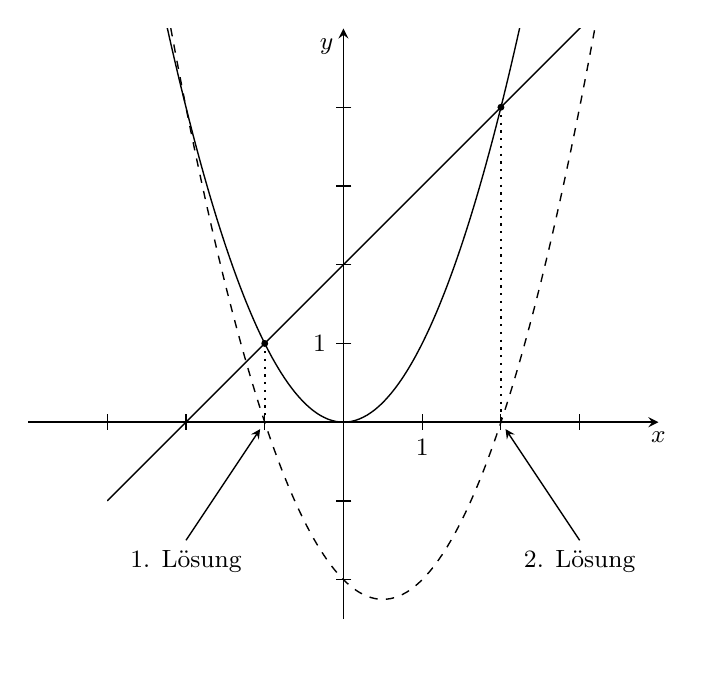
\begin{tikzpicture}
    % Koordinatenachsen
    \draw[line width=0.6pt, ->, >=stealth] (-4, 0) -- (4, 0) node[below] {{\small$x$}};
    \draw[line width=0.6pt, ->, >=stealth] (0, -2.5) -- (0, 5) node[below left] {{\small$y$}};
    % Skalierung der x-Achse
    \draw[xshift=-3cm] (0, 0.1) -- (0, -0.1);
    \draw[xshift=-2cm] (0, 0.1) -- (0, -0.1);
    \draw[xshift=-1cm] (0, 0.1) -- (0, -0.1);
    \draw[xshift= 1cm] (0, 0.1) -- (0, -0.1) node[below]{{\small$1$}};
    \draw[xshift= 2cm] (0, 0.1) -- (0, -0.1);
    \draw[xshift= 3cm] (0, 0.1) -- (0, -0.1);
    % Skalierung der y-Achse
    \draw[yshift=-2cm] (0.1, 0) -- (-0.1, 0);
    \draw[yshift=-1cm] (0.1, 0) -- (-0.1, 0);
    \draw[yshift= 1cm] (0.1, 0) -- (-0.1, 0) node[left]{{\small$1$}};
    \draw[yshift= 2cm] (0.1, 0) -- (-0.1, 0);
    \draw[yshift= 3cm] (0.1, 0) -- (-0.1, 0);
    \draw[yshift= 4cm] (0.1, 0) -- (-0.1, 0);
    % Graphen
    \begin{scope}
      \clip (-3.000, -3.000) rectangle (4.000, 5.000);
      \draw[line width=0.5pt, style=dashed] plot[smooth] coordinates
      {
        ( -3.000,  10.000)	        ( -2.900,   9.310)
        ( -2.800,   8.640)	        ( -2.700,   7.990)
        ( -2.600,   7.360)	        ( -2.500,   6.750)
        ( -2.400,   6.160)	        ( -2.300,   5.590)
        ( -2.200,   5.040)	        ( -2.100,   4.510)
        ( -2.000,   4.000)	        ( -1.900,   3.510)
        ( -1.800,   3.040)	        ( -1.700,   2.590)
        ( -1.600,   2.160)	        ( -1.500,   1.750)
        ( -1.400,   1.360)	        ( -1.300,   0.990)
        ( -1.200,   0.640)	        ( -1.100,   0.310)
        ( -1.000,   0.000)	        ( -0.900,  -0.290)
        ( -0.800,  -0.560)	        ( -0.700,  -0.810)
        ( -0.600,  -1.040)	        ( -0.500,  -1.250)
        ( -0.400,  -1.440)	        ( -0.300,  -1.610)
        ( -0.200,  -1.760)	        ( -0.100,  -1.890)
        (  0.000,  -2.000)	        (  0.100,  -2.090)
        (  0.200,  -2.160)	        (  0.300,  -2.210)
        (  0.400,  -2.240)	        (  0.500,  -2.250)
        (  0.600,  -2.240)	        (  0.700,  -2.210)
        (  0.800,  -2.160)	        (  0.900,  -2.090)
        (  1.000,  -2.000)	        (  1.100,  -1.890)
        (  1.200,  -1.760)	        (  1.300,  -1.610)
        (  1.400,  -1.440)	        (  1.500,  -1.250)
        (  1.600,  -1.040)	        (  1.700,  -0.810)
        (  1.800,  -0.560)	        (  1.900,  -0.290)
        (  2.000,   0.000)	        (  2.100,   0.310)
        (  2.200,   0.640)	        (  2.300,   0.990)
        (  2.400,   1.360)	        (  2.500,   1.750)
        (  2.600,   2.160)	        (  2.700,   2.590)
        (  2.800,   3.040)	        (  2.900,   3.510)
        (  3.000,   4.000)	        (  3.100,   4.510)
        (  3.200,   5.040)	        (  3.300,   5.590)
        (  3.400,   6.160)	        (  3.500,   6.750)
        (  3.600,   7.360)	        (  3.700,   7.990)
        (  3.800,   8.640)	        (  3.900,   9.310)
        (  4.000,  10.000)
      };
    \end{scope}
    \begin{scope}
      \clip (-3.000, -3.000) rectangle (4.000, 5.000);
      \draw[line width=0.5pt] plot[smooth] coordinates
      {
        ( -3.000,   9.000)	        ( -2.900,   8.410)
        ( -2.800,   7.840)	        ( -2.700,   7.290)
        ( -2.600,   6.760)	        ( -2.500,   6.250)
        ( -2.400,   5.760)	        ( -2.300,   5.290)
        ( -2.200,   4.840)	        ( -2.100,   4.410)
        ( -2.000,   4.000)	        ( -1.900,   3.610)
        ( -1.800,   3.240)	        ( -1.700,   2.890)
        ( -1.600,   2.560)	        ( -1.500,   2.250)
        ( -1.400,   1.960)	        ( -1.300,   1.690)
        ( -1.200,   1.440)	        ( -1.100,   1.210)
        ( -1.000,   1.000)	        ( -0.900,   0.810)
        ( -0.800,   0.640)	        ( -0.700,   0.490)
        ( -0.600,   0.360)	        ( -0.500,   0.250)
        ( -0.400,   0.160)	        ( -0.300,   0.090)
        ( -0.200,   0.040)	        ( -0.100,   0.010)
        (  0.000,   0.000)	        (  0.100,   0.010)
        (  0.200,   0.040)	        (  0.300,   0.090)
        (  0.400,   0.160)	        (  0.500,   0.250)
        (  0.600,   0.360)	        (  0.700,   0.490)
        (  0.800,   0.640)	        (  0.900,   0.810)
        (  1.000,   1.000)	        (  1.100,   1.210)
        (  1.200,   1.440)	        (  1.300,   1.690)
        (  1.400,   1.960)	        (  1.500,   2.250)
        (  1.600,   2.560)	        (  1.700,   2.890)
        (  1.800,   3.240)	        (  1.900,   3.610)
        (  2.000,   4.000)	        (  2.100,   4.410)
        (  2.200,   4.840)	        (  2.300,   5.290)
        (  2.400,   5.760)	        (  2.500,   6.250)
        (  2.600,   6.760)	        (  2.700,   7.290)
        (  2.800,   7.840)	        (  2.900,   8.410)
        (  3.000,   9.000)	        (  3.100,   9.610)
        (  3.200,  10.240)	        (  3.300,  10.890)
        (  3.400,  11.560)	        (  3.500,  12.250)
        (  3.600,  12.960)	        (  3.700,  13.690)
        (  3.800,  14.440)	        (  3.900,  15.210)
        (  4.000,  16.000)
      };
    \end{scope}
    \begin{scope}
      \clip (-3.000, -3.000) rectangle (4.000, 5.000);
      \draw[line width=0.5pt] (-3.000, -1.000) -- (4.000, 6.000);
    \end{scope}
    % Schnittpunkte
    \fill (-1, 1) circle[radius=1.25pt];
    \fill ( 2, 4) circle[radius=1.25pt];
    % Hilfslinien
    \draw[line width=0.8pt, style=dotted] ( 2, 4) -- ( 2, 0);
    \draw[line width=0.8pt, style=dotted] (-1, 1) -- (-1, 0);
    % Beschriftung
    \draw[line width=0.5pt, <-, >=stealth, shorten <=3pt] (-1, 0) -- (-2, -1.5) node[below]{{\small 1. Lösung}};;
    \draw[line width=0.5pt, <-, >=stealth, shorten <=3pt] ( 2, 0) -- ( 3, -1.5) node[below]{{\small 2. Lösung}};;
  \end{tikzpicture}
\end{center}

% -----------------
\paragraph{Aufgabe}
% -----------------
Bestimme die Nullstellen der Parabeln grafisch:
\paragraph{Rationale Koeffizienten und Lösungen}
\setvstrut{$\displaystyle(\frac{0}{1})$}%
\allowdisplaybreaks
\begin{alignat*}{5}
  \text{01)}\qquad f(x)&=-\frac{\num{243}}{\num{64}}x^{\num{2}}-\frac{\num{27}}{\num{32}}x+\frac{\num{189}}{\num{64}} & \colgap & \text{NST}&=\left\{\num{-1};\frac{\num{7}}{\num{9}}\right\} & \colgap & S&\left(-\frac{\num{1}}{\num{9}}\;\middle|\;\num{3}\right) \\[1ex]
  \text{02)}\qquad f(x)&=\frac{\num{175}}{\num{432}}x^{\num{2}}-\frac{\num{35}}{\num{108}}x-\frac{\num{245}}{\num{108}} & \colgap & \text{NST}&=\left\{\num{-2};\frac{\num{14}}{\num{5}}\right\} & \colgap & S&\left(\frac{\num{2}}{\num{5}}\;\middle|\;-\frac{\num{7}}{\num{3}}\right) \\[1ex]
  \text{03)}\qquad f(x)&=\frac{\num{99}}{\num{32}}x^{\num{2}}-\frac{\num{77}}{\num{16}}x-\frac{\num{55}}{\num{96}} & \colgap & \text{NST}&=\left\{-\frac{\num{1}}{\num{9}};\frac{\num{5}}{\num{3}}\right\} & \colgap & S&\left(\frac{\num{7}}{\num{9}}\;\middle|\;-\frac{\num{22}}{\num{9}}\right) \\[1ex]
  \text{04)}\qquad f(x)&=-\frac{\num{75}}{\num{128}}x^{\num{2}}+\frac{\num{45}}{\num{16}}x-\frac{\num{15}}{\num{8}} & \colgap & \text{NST}&=\left\{\frac{\num{4}}{\num{5}};\num{4}\right\} & \colgap & S&\left(\frac{\num{12}}{\num{5}}\;\middle|\;\frac{\num{3}}{\num{2}}\right) \\[1ex]
  \text{05)}\qquad f(x)&=-\frac{\num{11}}{\num{12}}x^{\num{2}}-\frac{\num{143}}{\num{54}}x+\sqrt{\frac{\num{40}}{\num{13}}} & \colgap & \text{NST}&=\left\{-\frac{\num{31}}{\num{9}};\frac{\num{5}}{\num{9}}\right\} & \colgap & S&\left(-\frac{\num{13}}{\num{9}}\;\middle|\;\frac{\num{11}}{\num{3}}\right) \\[1ex]
  \text{06)}\qquad f(x)&=-\frac{\num{112}}{\num{529}}x^{\num{2}}-\frac{\num{196}}{\num{529}}x+\frac{\num{840}}{\num{529}} & \colgap & \text{NST}&=\left\{-\frac{\num{15}}{\num{4}};\num{2}\right\} & \colgap & S&\left(-\frac{\num{7}}{\num{8}}\;\middle|\;\frac{\num{7}}{\num{4}}\right) \\[1ex]
  \text{07)}\qquad f(x)&=\frac{\num{4}}{\num{45}}x^{\num{2}}+\frac{\num{4}}{\num{45}}x-\frac{\num{8}}{\num{15}} & \colgap & \text{NST}&=\left\{\num{-3};\num{2}\right\} & \colgap & S&\left(-\frac{\num{1}}{\num{2}}\;\middle|\;-\frac{\num{5}}{\num{9}}\right) \\[1ex]
  \text{08)}\qquad f(x)&=\num{36}x^{\num{2}}-\num{204}x+\num{288} & \colgap & \text{NST}&=\left\{\frac{\num{8}}{\num{3}};\num{3}\right\} & \colgap & S&\left(\frac{\num{17}}{\num{6}}\;\middle|\;\num{-1}\right) \\[1ex]
  \text{09)}\qquad f(x)&=-\frac{\num{112}}{\num{27}}x^{\num{2}}+\frac{\num{280}}{\num{9}}x-\num{56} & \colgap & \text{NST}&=\left\{\num{3};\frac{\num{9}}{\num{2}}\right\} & \colgap & S&\left(\frac{\num{15}}{\num{4}}\;\middle|\;\frac{\num{7}}{\num{3}}\right) \\[1ex]
  \text{10)}\qquad f(x)&=-\frac{\num{232}}{\num{363}}x^{\num{2}}+\frac{\num{348}}{\num{121}}x+\frac{\num{580}}{\num{363}} & \colgap & \text{NST}&=\left\{-\frac{\num{1}}{\num{2}};\num{5}\right\} & \colgap & S&\left(\frac{\num{9}}{\num{4}}\;\middle|\;\frac{\num{29}}{\num{6}}\right) \\[1ex]
  \text{11)}\qquad f(x)&=-\frac{\num{48}}{\num{49}}x^{\num{2}}+\frac{\num{80}}{\num{49}}x+\frac{\num{32}}{\num{49}} & \colgap & \text{NST}&=\left\{-\frac{\num{1}}{\num{3}};\num{2}\right\} & \colgap & S&\left(\frac{\num{5}}{\num{6}}\;\middle|\;\frac{\num{4}}{\num{3}}\right) \\[1ex]
  \text{12)}\qquad f(x)&=\frac{\num{144}}{\num{13}}x^{\num{2}}-\frac{\num{536}}{\num{13}}x+\frac{\num{480}}{\num{13}} & \colgap & \text{NST}&=\left\{\frac{\num{3}}{\num{2}};\frac{\num{20}}{\num{9}}\right\} & \colgap & S&\left(\frac{\num{67}}{\num{36}}\;\middle|\;-\frac{\num{13}}{\num{9}}\right) \\[1ex]
  \text{13)}\qquad f(x)&=-\frac{\num{48}}{\num{49}}x^{\num{2}}-\frac{\num{40}}{\num{49}}x+\frac{\num{416}}{\num{147}} & \colgap & \text{NST}&=\left\{-\frac{\num{13}}{\num{6}};\frac{\num{4}}{\num{3}}\right\} & \colgap & S&\left(-\frac{\num{5}}{\num{12}}\;\middle|\;\num{3}\right) \\[1ex]
  \text{14)}\qquad f(x)&=-\frac{\num{256}}{\num{81}}x^{\num{2}}-\frac{\num{64}}{\num{81}}x+\frac{\num{320}}{\num{81}} & \colgap & \text{NST}&=\left\{-\frac{\num{5}}{\num{4}};\num{1}\right\} & \colgap & S&\left(-\frac{\num{1}}{\num{8}}\;\middle|\;\num{4}\right) \\[1ex]
  \text{15)}\qquad f(x)&=-\frac{\num{24}}{\num{289}}x^{\num{2}}+\frac{\num{32}}{\num{289}}x+\frac{\num{182}}{\num{289}} & \colgap & \text{NST}&=\left\{-\frac{\num{13}}{\num{6}};\frac{\num{7}}{\num{2}}\right\} & \colgap & S&\left(\frac{\num{2}}{\num{3}}\;\middle|\;\frac{\num{2}}{\num{3}}\right) \\[1ex]
  \text{16)}\qquad f(x)&=\frac{\num{15}}{\num{16}}x^{\num{2}}+\frac{\num{45}}{\num{16}}x-\frac{\num{105}}{\num{64}} & \colgap & \text{NST}&=\left\{-\frac{\num{7}}{\num{2}};\frac{\num{1}}{\num{2}}\right\} & \colgap & S&\left(-\frac{\num{3}}{\num{2}}\;\middle|\;-\frac{\num{15}}{\num{4}}\right) \\[1ex]
  \text{17)}\qquad f(x)&=-\frac{\num{189}}{\num{128}}x^{\num{2}}+\frac{\num{105}}{\num{64}}x+\frac{\num{91}}{\num{128}} & \colgap & \text{NST}&=\left\{-\frac{\num{1}}{\num{3}};\frac{\num{13}}{\num{9}}\right\} & \colgap & S&\left(\frac{\num{5}}{\num{9}}\;\middle|\;\frac{\num{7}}{\num{6}}\right) \\[1ex]
  \text{18)}\qquad f(x)&=\frac{\num{5}}{\num{6}}x^{\num{2}}-\num{6}x+\frac{\num{299}}{\num{30}} & \colgap & \text{NST}&=\left\{\frac{\num{13}}{\num{5}};\frac{\num{23}}{\num{5}}\right\} & \colgap & S&\left(\frac{\num{18}}{\num{5}}\;\middle|\;-\frac{\num{5}}{\num{6}}\right) \\[1ex]
  \text{19)}\qquad f(x)&=-\frac{\num{400}}{\num{121}}x^{\num{2}}-\frac{\num{80}}{\num{121}}x+\frac{\num{480}}{\num{121}} & \colgap & \text{NST}&=\left\{-\frac{\num{6}}{\num{5}};\num{1}\right\} & \colgap & S&\left(-\frac{\num{1}}{\num{10}}\;\middle|\;\num{4}\right) \\[1ex]
  \text{20)}\qquad f(x)&=-\frac{\num{243}}{\num{80}}x^{\num{2}}-\frac{\num{27}}{\num{2}}x-\frac{\num{63}}{\num{5}} & \colgap & \text{NST}&=\left\{-\frac{\num{28}}{\num{9}};-\frac{\num{4}}{\num{3}}\right\} & \colgap & S&\left(-\frac{\num{20}}{\num{9}}\;\middle|\;\frac{\num{12}}{\num{5}}\right) \\[1ex]
  \text{21)}\qquad f(x)&=\frac{\num{3}}{\num{2}}x^{\num{2}}-\frac{\num{23}}{\num{3}}x+\frac{\num{385}}{\num{54}} & \colgap & \text{NST}&=\left\{\frac{\num{11}}{\num{9}};\frac{\num{35}}{\num{9}}\right\} & \colgap & S&\left(\frac{\num{23}}{\num{9}}\;\middle|\;-\frac{\num{8}}{\num{3}}\right) \\[1ex]
  \text{22)}\qquad f(x)&=-\frac{\num{208}}{\num{625}}x^{\num{2}}-\sqrt{\frac{\num{842}}{\num{947}}}x+\sqrt{\frac{\num{281}}{\num{466}}} & \colgap & \text{NST}&=\left\{-\frac{\num{7}}{\num{2}};\frac{\num{2}}{\num{3}}\right\} & \colgap & S&\left(-\frac{\num{17}}{\num{12}}\;\middle|\;\frac{\num{13}}{\num{9}}\right) \\[1ex]
  \text{23)}\qquad f(x)&=-\frac{\num{25}}{\num{16}}x^{\num{2}}-\frac{\num{15}}{\num{8}}x+\frac{\num{55}}{\num{16}} & \colgap & \text{NST}&=\left\{-\frac{\num{11}}{\num{5}};\num{1}\right\} & \colgap & S&\left(-\frac{\num{3}}{\num{5}}\;\middle|\;\num{4}\right) \\[1ex]
  \text{24)}\qquad f(x)&=\frac{\num{27}}{\num{32}}x^{\num{2}}+\frac{\num{63}}{\num{16}}x+\frac{\num{99}}{\num{32}} & \colgap & \text{NST}&=\left\{-\frac{\num{11}}{\num{3}};\num{-1}\right\} & \colgap & S&\left(-\frac{\num{7}}{\num{3}}\;\middle|\;-\frac{\num{3}}{\num{2}}\right) \\[1ex]
  \text{25)}\qquad f(x)&=\num{475}x^{\num{2}}+\num{2185}x+\num{2508} & \colgap & \text{NST}&=\left\{-\frac{\num{12}}{\num{5}};-\frac{\num{11}}{\num{5}}\right\} & \colgap & S&\left(-\frac{\num{23}}{\num{10}}\;\middle|\;-\frac{\num{19}}{\num{4}}\right) \\[1ex]
  \text{26)}\qquad f(x)&=\frac{\num{5}}{\num{4}}x^{\num{2}}-\frac{\num{15}}{\num{2}}x+\frac{\num{25}}{\num{4}} & \colgap & \text{NST}&=\left\{\num{1};\num{5}\right\} & \colgap & S&\left(\num{3}\;\middle|\;\num{-5}\right) \\[1ex]
  \text{27)}\qquad f(x)&=\frac{\num{1}}{\num{4}}x^{\num{2}}-\num{1} & \colgap & \text{NST}&=\left\{\num{-2};\num{2}\right\} & \colgap & S&\left(\num{0}\;\middle|\;\num{-1}\right) \\[1ex]
  \text{28)}\qquad f(x)&=-\frac{\num{162}}{\num{5}}x^{\num{2}}-\frac{\num{468}}{\num{5}}x-\num{66} & \colgap & \text{NST}&=\left\{-\frac{\num{5}}{\num{3}};-\frac{\num{11}}{\num{9}}\right\} & \colgap & S&\left(-\frac{\num{13}}{\num{9}}\;\middle|\;\frac{\num{8}}{\num{5}}\right) \\[1ex]
  \text{29)}\qquad f(x)&=-\frac{\num{27}}{\num{100}}x^{\num{2}}-\frac{\num{9}}{\num{10}}x+\frac{\num{9}}{\num{4}} & \colgap & \text{NST}&=\left\{\num{-5};\frac{\num{5}}{\num{3}}\right\} & \colgap & S&\left(-\frac{\num{5}}{\num{3}}\;\middle|\;\num{3}\right) \\[1ex]
  \text{30)}\qquad f(x)&=\frac{\num{432}}{\num{289}}x^{\num{2}}+\frac{\num{936}}{\num{289}}x-\frac{\num{360}}{\num{289}} & \colgap & \text{NST}&=\left\{-\frac{\num{5}}{\num{2}};\frac{\num{1}}{\num{3}}\right\} & \colgap & S&\left(-\frac{\num{13}}{\num{12}}\;\middle|\;\num{-3}\right) \\[1ex]
  \text{31)}\qquad f(x)&=\frac{\num{36}}{\num{5}}x^{\num{2}}+\frac{\num{228}}{\num{5}}x+\num{72} & \colgap & \text{NST}&=\left\{-\frac{\num{10}}{\num{3}};\num{-3}\right\} & \colgap & S&\left(-\frac{\num{19}}{\num{6}}\;\middle|\;-\frac{\num{1}}{\num{5}}\right) \\[1ex]
  \text{32)}\qquad f(x)&=-\frac{\num{88}}{\num{169}}x^{\num{2}}+\frac{\num{440}}{\num{507}}x+\frac{\num{352}}{\num{169}} & \colgap & \text{NST}&=\left\{-\frac{\num{4}}{\num{3}};\num{3}\right\} & \colgap & S&\left(\frac{\num{5}}{\num{6}}\;\middle|\;\frac{\num{22}}{\num{9}}\right) \\[1ex]
  \text{33)}\qquad f(x)&=-\frac{\num{64}}{\num{49}}x^{\num{2}}-\frac{\num{96}}{\num{49}}x+\frac{\num{160}}{\num{49}} & \colgap & \text{NST}&=\left\{-\frac{\num{5}}{\num{2}};\num{1}\right\} & \colgap & S&\left(-\frac{\num{3}}{\num{4}}\;\middle|\;\num{4}\right) \\[1ex]
  \text{34)}\qquad f(x)&=\frac{\num{432}}{\num{25}}x^{\num{2}}-\frac{\num{72}}{\num{25}}x-\frac{\num{72}}{\num{25}} & \colgap & \text{NST}&=\left\{-\frac{\num{1}}{\num{3}};\frac{\num{1}}{\num{2}}\right\} & \colgap & S&\left(\frac{\num{1}}{\num{12}}\;\middle|\;\num{-3}\right) \\[1ex]
  \text{35)}\qquad f(x)&=\frac{\num{32}}{\num{13}}x^{\num{2}}-\frac{\num{656}}{\num{39}}x+\frac{\num{336}}{\num{13}} & \colgap & \text{NST}&=\left\{\frac{\num{7}}{\num{3}};\frac{\num{9}}{\num{2}}\right\} & \colgap & S&\left(\frac{\num{41}}{\num{12}}\;\middle|\;-\frac{\num{26}}{\num{9}}\right) \\[1ex]
  \text{36)}\qquad f(x)&=-\frac{\num{879}}{\num{719}}x^{\num{2}}-\frac{\num{331}}{\num{171}}x+\frac{\num{662}}{\num{361}} & \colgap & \text{NST}&=\left\{-\frac{\num{9}}{\num{4}};\frac{\num{2}}{\num{3}}\right\} & \colgap & S&\left(-\frac{\num{19}}{\num{24}}\;\middle|\;\frac{\num{13}}{\num{5}}\right) \\[1ex]
  \text{37)}\qquad f(x)&=-\frac{\num{324}}{\num{125}}x^{\num{2}}+\frac{\num{396}}{\num{125}}x+\frac{\num{504}}{\num{125}} & \colgap & \text{NST}&=\left\{-\frac{\num{7}}{\num{9}};\num{2}\right\} & \colgap & S&\left(\frac{\num{11}}{\num{18}}\;\middle|\;\num{5}\right) \\[1ex]
  \text{38)}\qquad f(x)&=\frac{\num{25}}{\num{14}}x^{\num{2}}+\frac{\num{60}}{\num{7}}x+\frac{\num{95}}{\num{14}} & \colgap & \text{NST}&=\left\{-\frac{\num{19}}{\num{5}};\num{-1}\right\} & \colgap & S&\left(-\frac{\num{12}}{\num{5}}\;\middle|\;-\frac{\num{7}}{\num{2}}\right) \\[1ex]
  \text{39)}\qquad f(x)&=-\frac{\num{135}}{\num{2}}x^{\num{2}}+\num{144}x-\num{72} & \colgap & \text{NST}&=\left\{\frac{\num{4}}{\num{5}};\frac{\num{4}}{\num{3}}\right\} & \colgap & S&\left(\frac{\num{16}}{\num{15}}\;\middle|\;\frac{\num{24}}{\num{5}}\right) \\[1ex]
  \text{40)}\qquad f(x)&=\frac{\num{28}}{\num{27}}x^{\num{2}}+\frac{\num{56}}{\num{27}}x-\frac{\num{35}}{\num{27}} & \colgap & \text{NST}&=\left\{-\frac{\num{5}}{\num{2}};\frac{\num{1}}{\num{2}}\right\} & \colgap & S&\left(\num{-1}\;\middle|\;-\frac{\num{7}}{\num{3}}\right) \\[1ex]
  \text{41)}\qquad f(x)&=-\num{60}x^{\num{2}}+\num{280}x-\num{325} & \colgap & \text{NST}&=\left\{\frac{\num{13}}{\num{6}};\frac{\num{5}}{\num{2}}\right\} & \colgap & S&\left(\frac{\num{7}}{\num{3}}\;\middle|\;\frac{\num{5}}{\num{3}}\right) \\[1ex]
  \text{42)}\qquad f(x)&=\frac{\num{9}}{\num{40}}x^{\num{2}}+\frac{\num{3}}{\num{4}}x+\frac{\num{9}}{\num{40}} & \colgap & \text{NST}&=\left\{\num{-3};-\frac{\num{1}}{\num{3}}\right\} & \colgap & S&\left(-\frac{\num{5}}{\num{3}}\;\middle|\;-\frac{\num{2}}{\num{5}}\right) \\[1ex]
  \text{43)}\qquad f(x)&=\frac{\num{405}}{\num{4}}x^{\num{2}}+\num{450}x+\num{495} & \colgap & \text{NST}&=\left\{-\frac{\num{22}}{\num{9}};\num{-2}\right\} & \colgap & S&\left(-\frac{\num{20}}{\num{9}}\;\middle|\;\num{-5}\right) \\[1ex]
  \text{44)}\qquad f(x)&=\frac{\num{9}}{\num{2}}x^{\num{2}}-\num{27}x+\num{36} & \colgap & \text{NST}&=\left\{\num{2};\num{4}\right\} & \colgap & S&\left(\num{3}\;\middle|\;-\frac{\num{9}}{\num{2}}\right) \\[1ex]
  \text{45)}\qquad f(x)&=\frac{\num{792}}{\num{289}}x^{\num{2}}-\frac{\num{88}}{\num{289}}x-\frac{\num{704}}{\num{289}} & \colgap & \text{NST}&=\left\{-\frac{\num{8}}{\num{9}};\num{1}\right\} & \colgap & S&\left(\frac{\num{1}}{\num{18}}\;\middle|\;-\frac{\num{22}}{\num{9}}\right) \\[1ex]
  \text{46)}\qquad f(x)&=\num{40}x^{\num{2}}-\num{60}x+\num{20} & \colgap & \text{NST}&=\left\{\frac{\num{1}}{\num{2}};\num{1}\right\} & \colgap & S&\left(\frac{\num{3}}{\num{4}}\;\middle|\;-\frac{\num{5}}{\num{2}}\right) \\[1ex]
  \text{47)}\qquad f(x)&=\frac{\num{72}}{\num{625}}x^{\num{2}}+\frac{\num{156}}{\num{625}}x-\frac{\num{228}}{\num{625}} & \colgap & \text{NST}&=\left\{-\frac{\num{19}}{\num{6}};\num{1}\right\} & \colgap & S&\left(-\frac{\num{13}}{\num{12}}\;\middle|\;-\frac{\num{1}}{\num{2}}\right) \\[1ex]
  \text{48)}\qquad f(x)&=\frac{\num{800}}{\num{121}}x^{\num{2}}-\frac{\num{840}}{\num{121}}x+\frac{\num{160}}{\num{121}} & \colgap & \text{NST}&=\left\{\frac{\num{1}}{\num{4}};\frac{\num{4}}{\num{5}}\right\} & \colgap & S&\left(\frac{\num{21}}{\num{40}}\;\middle|\;-\frac{\num{1}}{\num{2}}\right) \\[1ex]
  \text{49)}\qquad f(x)&=\frac{\num{7}}{\num{6}}x^{\num{2}}-\frac{\num{14}}{\num{3}} & \colgap & \text{NST}&=\left\{\num{-2};\num{2}\right\} & \colgap & S&\left(\num{0}\;\middle|\;-\frac{\num{14}}{\num{3}}\right) \\[1ex]
  \text{50)}\qquad f(x)&=-\frac{\num{3}}{\num{7}}x^{\num{2}}+\frac{\num{10}}{\num{7}}x+\frac{\num{8}}{\num{7}} & \colgap & \text{NST}&=\left\{-\frac{\num{2}}{\num{3}};\num{4}\right\} & \colgap & S&\left(\frac{\num{5}}{\num{3}}\;\middle|\;\frac{\num{7}}{\num{3}}\right) \\[1ex]
  \text{51)}\qquad f(x)&=\num{28}x^{\num{2}}-\frac{\num{224}}{\num{3}}x+\frac{\num{140}}{\num{3}} & \colgap & \text{NST}&=\left\{\num{1};\frac{\num{5}}{\num{3}}\right\} & \colgap & S&\left(\frac{\num{4}}{\num{3}}\;\middle|\;-\frac{\num{28}}{\num{9}}\right) \\[1ex]
  \text{52)}\qquad f(x)&=\frac{\num{900}}{\num{637}}x^{\num{2}}+\frac{\num{690}}{\num{91}}x+\frac{\num{90}}{\num{13}} & \colgap & \text{NST}&=\left\{-\frac{\num{21}}{\num{5}};-\frac{\num{7}}{\num{6}}\right\} & \colgap & S&\left(-\frac{\num{161}}{\num{60}}\;\middle|\;-\frac{\num{13}}{\num{4}}\right) \\[1ex]
  \text{53)}\qquad f(x)&=-\num{240}x^{\num{2}}-\num{1640}x-\num{2800} & \colgap & \text{NST}&=\left\{-\frac{\num{7}}{\num{2}};-\frac{\num{10}}{\num{3}}\right\} & \colgap & S&\left(-\frac{\num{41}}{\num{12}}\;\middle|\;\frac{\num{5}}{\num{3}}\right) \\[1ex]
  \text{54)}\qquad f(x)&=\frac{\num{81}}{\num{640}}x^{\num{2}}+\frac{\num{9}}{\num{32}}x-\frac{\num{231}}{\num{160}} & \colgap & \text{NST}&=\left\{-\frac{\num{14}}{\num{3}};\frac{\num{22}}{\num{9}}\right\} & \colgap & S&\left(-\frac{\num{10}}{\num{9}}\;\middle|\;-\frac{\num{8}}{\num{5}}\right) \\[1ex]
  \text{55)}\qquad f(x)&=\frac{\num{99}}{\num{100}}x^{\num{2}}+\frac{\num{121}}{\num{25}}x+\frac{\num{352}}{\num{75}} & \colgap & \text{NST}&=\left\{-\frac{\num{32}}{\num{9}};-\frac{\num{4}}{\num{3}}\right\} & \colgap & S&\left(-\frac{\num{22}}{\num{9}}\;\middle|\;-\frac{\num{11}}{\num{9}}\right) \\[1ex]
  \text{56)}\qquad f(x)&=\num{171}x^{\num{2}}+\num{1064}x+\num{1653} & \colgap & \text{NST}&=\left\{-\frac{\num{29}}{\num{9}};\num{-3}\right\} & \colgap & S&\left(-\frac{\num{28}}{\num{9}}\;\middle|\;-\frac{\num{19}}{\num{9}}\right) \\[1ex]
  \text{57)}\qquad f(x)&=\frac{\num{162}}{\num{529}}x^{\num{2}}-\frac{\num{882}}{\num{529}}x+\frac{\num{936}}{\num{529}} & \colgap & \text{NST}&=\left\{\frac{\num{13}}{\num{9}};\num{4}\right\} & \colgap & S&\left(\frac{\num{49}}{\num{18}}\;\middle|\;-\frac{\num{1}}{\num{2}}\right) \\[1ex]
  \text{58)}\qquad f(x)&=-\frac{\num{864}}{\num{169}}x^{\num{2}}+\frac{\num{504}}{\num{13}}x-\num{72} & \colgap & \text{NST}&=\left\{\frac{\num{13}}{\num{4}};\frac{\num{13}}{\num{3}}\right\} & \colgap & S&\left(\frac{\num{91}}{\num{24}}\;\middle|\;\frac{\num{3}}{\num{2}}\right) \\[1ex]
  \text{59)}\qquad f(x)&=\frac{\num{36}}{\num{25}}x^{\num{2}}+\frac{\num{216}}{\num{25}}x+\frac{\num{224}}{\num{25}} & \colgap & \text{NST}&=\left\{-\frac{\num{14}}{\num{3}};-\frac{\num{4}}{\num{3}}\right\} & \colgap & S&\left(\num{-3}\;\middle|\;\num{-4}\right) \\[1ex]
  \text{60)}\qquad f(x)&=-\frac{\num{4}}{\num{9}}x^{\num{2}}+\frac{\num{20}}{\num{9}}x-\frac{\num{16}}{\num{9}} & \colgap & \text{NST}&=\left\{\num{1};\num{4}\right\} & \colgap & S&\left(\frac{\num{5}}{\num{2}}\;\middle|\;\num{1}\right) \\[1ex]
  \text{61)}\qquad f(x)&=-\frac{\num{11}}{\num{18}}x^{\num{2}}+\frac{\num{77}}{\num{27}}x-\frac{\num{143}}{\num{162}} & \colgap & \text{NST}&=\left\{\frac{\num{1}}{\num{3}};\frac{\num{13}}{\num{3}}\right\} & \colgap & S&\left(\frac{\num{7}}{\num{3}}\;\middle|\;\frac{\num{22}}{\num{9}}\right) \\[1ex]
  \text{62)}\qquad f(x)&=\frac{\num{250}}{\num{81}}x^{\num{2}}+\frac{\num{100}}{\num{9}}x+\frac{\num{50}}{\num{9}} & \colgap & \text{NST}&=\left\{\num{-3};-\frac{\num{3}}{\num{5}}\right\} & \colgap & S&\left(-\frac{\num{9}}{\num{5}}\;\middle|\;-\frac{\num{40}}{\num{9}}\right) \\[1ex]
  \text{63)}\qquad f(x)&=\frac{\num{4}}{\num{49}}x^{\num{2}}+\frac{\num{16}}{\num{147}}x-\frac{\num{20}}{\num{49}} & \colgap & \text{NST}&=\left\{\num{-3};\frac{\num{5}}{\num{3}}\right\} & \colgap & S&\left(-\frac{\num{2}}{\num{3}}\;\middle|\;-\frac{\num{4}}{\num{9}}\right) \\[1ex]
  \text{64)}\qquad f(x)&=-\frac{\num{54}}{\num{169}}x^{\num{2}}-\frac{\num{102}}{\num{169}}x+\frac{\num{616}}{\num{507}} & \colgap & \text{NST}&=\left\{-\frac{\num{28}}{\num{9}};\frac{\num{11}}{\num{9}}\right\} & \colgap & S&\left(-\frac{\num{17}}{\num{18}}\;\middle|\;\frac{\num{3}}{\num{2}}\right) \\[1ex]
  \text{65)}\qquad f(x)&=-\frac{\num{2}}{\num{21}}x^{\num{2}}-\frac{\num{10}}{\num{63}}x+\frac{\num{208}}{\num{189}} & \colgap & \text{NST}&=\left\{-\frac{\num{13}}{\num{3}};\frac{\num{8}}{\num{3}}\right\} & \colgap & S&\left(-\frac{\num{5}}{\num{6}}\;\middle|\;\frac{\num{7}}{\num{6}}\right) \\[1ex]
  \text{66)}\qquad f(x)&=-\frac{\num{297}}{\num{2}}x^{\num{2}}+\num{1023}x-\num{1760} & \colgap & \text{NST}&=\left\{\frac{\num{10}}{\num{3}};\frac{\num{32}}{\num{9}}\right\} & \colgap & S&\left(\frac{\num{31}}{\num{9}}\;\middle|\;\frac{\num{11}}{\num{6}}\right) \\[1ex]
  \text{67)}\qquad f(x)&=\frac{\num{2}}{\num{7}}x^{\num{2}}-\frac{\num{2}}{\num{7}}x-\frac{\num{24}}{\num{7}} & \colgap & \text{NST}&=\left\{\num{-3};\num{4}\right\} & \colgap & S&\left(\frac{\num{1}}{\num{2}}\;\middle|\;-\frac{\num{7}}{\num{2}}\right) \\[1ex]
  \text{68)}\qquad f(x)&=\frac{\num{41}}{\num{100}}x^{\num{2}}-\frac{\num{41}}{\num{150}}x-\frac{\num{451}}{\num{100}} & \colgap & \text{NST}&=\left\{\num{-3};\frac{\num{11}}{\num{3}}\right\} & \colgap & S&\left(\frac{\num{1}}{\num{3}}\;\middle|\;-\frac{\num{41}}{\num{9}}\right) \\[1ex]
  \text{69)}\qquad f(x)&=-\frac{\num{48}}{\num{169}}x^{\num{2}}+\frac{\num{184}}{\num{169}}x-\frac{\num{120}}{\num{169}} & \colgap & \text{NST}&=\left\{\frac{\num{5}}{\num{6}};\num{3}\right\} & \colgap & S&\left(\frac{\num{23}}{\num{12}}\;\middle|\;\frac{\num{1}}{\num{3}}\right) \\[1ex]
  \text{70)}\qquad f(x)&=-\frac{\num{36}}{\num{25}}x^{\num{2}}-\frac{\num{192}}{\num{25}}x-\frac{\num{156}}{\num{25}} & \colgap & \text{NST}&=\left\{-\frac{\num{13}}{\num{3}};\num{-1}\right\} & \colgap & S&\left(-\frac{\num{8}}{\num{3}}\;\middle|\;\num{4}\right) \\[1ex]
  \text{71)}\qquad f(x)&=\num{20}x^{\num{2}}-\frac{\num{260}}{\num{3}}x+\frac{\num{280}}{\num{3}} & \colgap & \text{NST}&=\left\{\num{2};\frac{\num{7}}{\num{3}}\right\} & \colgap & S&\left(\frac{\num{13}}{\num{6}}\;\middle|\;-\frac{\num{5}}{\num{9}}\right) \\[1ex]
  \text{72)}\qquad f(x)&=\num{144}x^{\num{2}}-\num{72}x+\num{8} & \colgap & \text{NST}&=\left\{\frac{\num{1}}{\num{6}};\frac{\num{1}}{\num{3}}\right\} & \colgap & S&\left(\frac{\num{1}}{\num{4}}\;\middle|\;\num{-1}\right) \\[1ex]
  \text{73)}\qquad f(x)&=-\frac{\num{81}}{\num{196}}x^{\num{2}}+\frac{\num{36}}{\num{49}}x+\frac{\num{33}}{\num{49}} & \colgap & \text{NST}&=\left\{-\frac{\num{2}}{\num{3}};\frac{\num{22}}{\num{9}}\right\} & \colgap & S&\left(\frac{\num{8}}{\num{9}}\;\middle|\;\num{1}\right) \\[1ex]
  \text{74)}\qquad f(x)&=\frac{\num{14}}{\num{5}}x^{\num{2}}+\frac{\num{84}}{\num{5}}x+\frac{\num{112}}{\num{5}} & \colgap & \text{NST}&=\left\{\num{-4};\num{-2}\right\} & \colgap & S&\left(\num{-3}\;\middle|\;-\frac{\num{14}}{\num{5}}\right) \\[1ex]
  \text{75)}\qquad f(x)&=-\num{60}x^{\num{2}}-\num{90}x-\num{30} & \colgap & \text{NST}&=\left\{\num{-1};-\frac{\num{1}}{\num{2}}\right\} & \colgap & S&\left(-\frac{\num{3}}{\num{4}}\;\middle|\;\frac{\num{15}}{\num{4}}\right) \\[1ex]
  \text{76)}\qquad f(x)&=-\frac{\num{81}}{\num{49}}x^{\num{2}}+\frac{\num{18}}{\num{49}}x+\frac{\num{48}}{\num{49}} & \colgap & \text{NST}&=\left\{-\frac{\num{2}}{\num{3}};\frac{\num{8}}{\num{9}}\right\} & \colgap & S&\left(\frac{\num{1}}{\num{9}}\;\middle|\;\num{1}\right) \\[1ex]
  \text{77)}\qquad f(x)&=-\frac{\num{20}}{\num{63}}x^{\num{2}}-\frac{\num{40}}{\num{63}}x+\frac{\num{25}}{\num{7}} & \colgap & \text{NST}&=\left\{-\frac{\num{9}}{\num{2}};\frac{\num{5}}{\num{2}}\right\} & \colgap & S&\left(\num{-1}\;\middle|\;\frac{\num{35}}{\num{9}}\right) \\[1ex]
  \text{78)}\qquad f(x)&=-\frac{\num{3}}{\num{4}}x^{\num{2}}-\num{2}x-\num{1} & \colgap & \text{NST}&=\left\{\num{-2};-\frac{\num{2}}{\num{3}}\right\} & \colgap & S&\left(-\frac{\num{4}}{\num{3}}\;\middle|\;\frac{\num{1}}{\num{3}}\right) \\[1ex]
  \text{79)}\qquad f(x)&=\frac{\num{144}}{\num{5}}x^{\num{2}}-\frac{\num{912}}{\num{5}}x+\num{288} & \colgap & \text{NST}&=\left\{\num{3};\frac{\num{10}}{\num{3}}\right\} & \colgap & S&\left(\frac{\num{19}}{\num{6}}\;\middle|\;-\frac{\num{4}}{\num{5}}\right) \\[1ex]
  \text{80)}\qquad f(x)&=\frac{\num{375}}{\num{98}}x^{\num{2}}-\num{25}x+\frac{\num{75}}{\num{2}} & \colgap & \text{NST}&=\left\{\frac{\num{7}}{\num{3}};\frac{\num{21}}{\num{5}}\right\} & \colgap & S&\left(\frac{\num{49}}{\num{15}}\;\middle|\;-\frac{\num{10}}{\num{3}}\right) \\[1ex]
  \text{81)}\qquad f(x)&=\num{28}x^{\num{2}}+\num{182}x+\num{294} & \colgap & \text{NST}&=\left\{-\frac{\num{7}}{\num{2}};\num{-3}\right\} & \colgap & S&\left(-\frac{\num{13}}{\num{4}}\;\middle|\;-\frac{\num{7}}{\num{4}}\right) \\[1ex]
  \text{82)}\qquad f(x)&=\frac{\num{425}}{\num{36}}x^{\num{2}}+\frac{\num{170}}{\num{3}}x+\frac{\num{255}}{\num{4}} & \colgap & \text{NST}&=\left\{\num{-3};-\frac{\num{9}}{\num{5}}\right\} & \colgap & S&\left(-\frac{\num{12}}{\num{5}}\;\middle|\;-\frac{\num{17}}{\num{4}}\right) \\[1ex]
  \text{83)}\qquad f(x)&=\num{72}x^{\num{2}}+\num{108}x+\num{36} & \colgap & \text{NST}&=\left\{\num{-1};-\frac{\num{1}}{\num{2}}\right\} & \colgap & S&\left(-\frac{\num{3}}{\num{4}}\;\middle|\;-\frac{\num{9}}{\num{2}}\right) \\[1ex]
  \text{84)}\qquad f(x)&=\frac{\num{9}}{\num{49}}x^{\num{2}}+\frac{\num{69}}{\num{49}}x+\frac{\num{120}}{\num{49}} & \colgap & \text{NST}&=\left\{\num{-5};-\frac{\num{8}}{\num{3}}\right\} & \colgap & S&\left(-\frac{\num{23}}{\num{6}}\;\middle|\;-\frac{\num{1}}{\num{4}}\right) \\[1ex]
  \text{85)}\qquad f(x)&=\frac{\num{1}}{\num{4}}x^{\num{2}}-\num{2}x+\frac{\num{15}}{\num{4}} & \colgap & \text{NST}&=\left\{\num{3};\num{5}\right\} & \colgap & S&\left(\num{4}\;\middle|\;-\frac{\num{1}}{\num{4}}\right) \\[1ex]
  \text{86)}\qquad f(x)&=-\frac{\num{16}}{\num{33}}x^{\num{2}}+\frac{\num{40}}{\num{33}}x+\frac{\num{32}}{\num{11}} & \colgap & \text{NST}&=\left\{-\frac{\num{3}}{\num{2}};\num{4}\right\} & \colgap & S&\left(\frac{\num{5}}{\num{4}}\;\middle|\;\frac{\num{11}}{\num{3}}\right) \\[1ex]
  \text{87)}\qquad f(x)&=-\frac{\num{176}}{\num{75}}x^{\num{2}}+\frac{\num{968}}{\num{75}}x-\frac{\num{352}}{\num{25}} & \colgap & \text{NST}&=\left\{\frac{\num{3}}{\num{2}};\num{4}\right\} & \colgap & S&\left(\frac{\num{11}}{\num{4}}\;\middle|\;\frac{\num{11}}{\num{3}}\right) \\[1ex]
  \text{88)}\qquad f(x)&=-\frac{\num{16}}{\num{121}}x^{\num{2}}-\frac{\num{24}}{\num{121}}x+\frac{\num{112}}{\num{121}} & \colgap & \text{NST}&=\left\{-\frac{\num{7}}{\num{2}};\num{2}\right\} & \colgap & S&\left(-\frac{\num{3}}{\num{4}}\;\middle|\;\num{1}\right) \\[1ex]
  \text{89)}\qquad f(x)&=-\frac{\num{184}}{\num{147}}x^{\num{2}}-\frac{\num{184}}{\num{147}}x+\frac{\num{345}}{\num{98}} & \colgap & \text{NST}&=\left\{-\frac{\num{9}}{\num{4}};\frac{\num{5}}{\num{4}}\right\} & \colgap & S&\left(-\frac{\num{1}}{\num{2}}\;\middle|\;\frac{\num{23}}{\num{6}}\right) \\[1ex]
  \text{90)}\qquad f(x)&=-\frac{\num{50}}{\num{169}}x^{\num{2}}+\frac{\num{160}}{\num{169}}x+\frac{\num{210}}{\num{169}} & \colgap & \text{NST}&=\left\{\num{-1};\frac{\num{21}}{\num{5}}\right\} & \colgap & S&\left(\frac{\num{8}}{\num{5}}\;\middle|\;\num{2}\right) \\[1ex]
  \text{91)}\qquad f(x)&=-\frac{\num{72}}{\num{289}}x^{\num{2}}+\frac{\num{48}}{\num{289}}x+\frac{\num{570}}{\num{289}} & \colgap & \text{NST}&=\left\{-\frac{\num{5}}{\num{2}};\frac{\num{19}}{\num{6}}\right\} & \colgap & S&\left(\frac{\num{1}}{\num{3}}\;\middle|\;\num{2}\right) \\[1ex]
  \text{92)}\qquad f(x)&=-\frac{\num{100}}{\num{81}}x^{\num{2}}-\frac{\num{40}}{\num{81}}x+\frac{\num{320}}{\num{81}} & \colgap & \text{NST}&=\left\{\num{-2};\frac{\num{8}}{\num{5}}\right\} & \colgap & S&\left(-\frac{\num{1}}{\num{5}}\;\middle|\;\num{4}\right) \\[1ex]
  \text{93)}\qquad f(x)&=\frac{\num{64}}{\num{75}}x^{\num{2}}+\frac{\num{64}}{\num{15}}x+\num{4} & \colgap & \text{NST}&=\left\{-\frac{\num{15}}{\num{4}};-\frac{\num{5}}{\num{4}}\right\} & \colgap & S&\left(-\frac{\num{5}}{\num{2}}\;\middle|\;-\frac{\num{4}}{\num{3}}\right) \\[1ex]
  \text{94)}\qquad f(x)&=-\frac{\num{20}}{\num{49}}x^{\num{2}}-\frac{\num{100}}{\num{147}}x+\frac{\num{40}}{\num{147}} & \colgap & \text{NST}&=\left\{\num{-2};\frac{\num{1}}{\num{3}}\right\} & \colgap & S&\left(-\frac{\num{5}}{\num{6}}\;\middle|\;\frac{\num{5}}{\num{9}}\right) \\[1ex]
  \text{95)}\qquad f(x)&=\frac{\num{14}}{\num{9}}x^{\num{2}}-\frac{\num{266}}{\num{27}}x+\frac{\num{980}}{\num{81}} & \colgap & \text{NST}&=\left\{\frac{\num{5}}{\num{3}};\frac{\num{14}}{\num{3}}\right\} & \colgap & S&\left(\frac{\num{19}}{\num{6}}\;\middle|\;-\frac{\num{7}}{\num{2}}\right) \\[1ex]
  \text{96)}\qquad f(x)&=\frac{\num{81}}{\num{256}}x^{\num{2}}+\frac{\num{9}}{\num{128}}x-\frac{\num{63}}{\num{256}} & \colgap & \text{NST}&=\left\{\num{-1};\frac{\num{7}}{\num{9}}\right\} & \colgap & S&\left(-\frac{\num{1}}{\num{9}}\;\middle|\;-\frac{\num{1}}{\num{4}}\right) \\[1ex]
  \text{97)}\qquad f(x)&=-\frac{\num{81}}{\num{4}}x^{\num{2}}+\num{180}x-\num{396} & \colgap & \text{NST}&=\left\{\num{4};\frac{\num{44}}{\num{9}}\right\} & \colgap & S&\left(\frac{\num{40}}{\num{9}}\;\middle|\;\num{4}\right) \\[1ex]
  \text{98)}\qquad f(x)&=-\frac{\num{168}}{\num{169}}x^{\num{2}}-\frac{\num{952}}{\num{169}}x-\frac{\num{560}}{\num{169}} & \colgap & \text{NST}&=\left\{\num{-5};-\frac{\num{2}}{\num{3}}\right\} & \colgap & S&\left(-\frac{\num{17}}{\num{6}}\;\middle|\;\frac{\num{14}}{\num{3}}\right) \\[1ex]
  \text{99)}\qquad f(x)&=\frac{\num{48}}{\num{169}}x^{\num{2}}+\frac{\num{180}}{\num{169}}x+\frac{\num{42}}{\num{169}} & \colgap & \text{NST}&=\left\{-\frac{\num{7}}{\num{2}};-\frac{\num{1}}{\num{4}}\right\} & \colgap & S&\left(-\frac{\num{15}}{\num{8}}\;\middle|\;-\frac{\num{3}}{\num{4}}\right) \\[1ex]
  \text{100)}\qquad f(x)&=\frac{\num{54}}{\num{7}}x^{\num{2}}-\frac{\num{156}}{\num{7}}x+\frac{\num{80}}{\num{7}} & \colgap & \text{NST}&=\left\{\frac{\num{2}}{\num{3}};\frac{\num{20}}{\num{9}}\right\} & \colgap & S&\left(\frac{\num{13}}{\num{9}}\;\middle|\;-\frac{\num{14}}{\num{3}}\right) \\[1ex]
  \text{101)}\qquad f(x)&=-\frac{\num{108}}{\num{5}}x^{\num{2}}+\frac{\num{414}}{\num{5}}x-\frac{\num{378}}{\num{5}} & \colgap & \text{NST}&=\left\{\frac{\num{3}}{\num{2}};\frac{\num{7}}{\num{3}}\right\} & \colgap & S&\left(\frac{\num{23}}{\num{12}}\;\middle|\;\frac{\num{15}}{\num{4}}\right) \\[1ex]
  \text{102)}\qquad f(x)&=-\frac{\num{320}}{\num{169}}x^{\num{2}}+\frac{\num{400}}{\num{169}}x+\frac{\num{720}}{\num{169}} & \colgap & \text{NST}&=\left\{\num{-1};\frac{\num{9}}{\num{4}}\right\} & \colgap & S&\left(\frac{\num{5}}{\num{8}}\;\middle|\;\num{5}\right) \\[1ex]
  \text{103)}\qquad f(x)&=-\frac{\num{32}}{\num{961}}x^{\num{2}}+\frac{\num{8}}{\num{961}}x+\frac{\num{480}}{\num{961}} & \colgap & \text{NST}&=\left\{-\frac{\num{15}}{\num{4}};\num{4}\right\} & \colgap & S&\left(\frac{\num{1}}{\num{8}}\;\middle|\;\frac{\num{1}}{\num{2}}\right) \\[1ex]
  \text{104)}\qquad f(x)&=\frac{\num{27}}{\num{125}}x^{\num{2}}-\frac{\num{18}}{\num{125}}x-\frac{\num{72}}{\num{125}} & \colgap & \text{NST}&=\left\{-\frac{\num{4}}{\num{3}};\num{2}\right\} & \colgap & S&\left(\frac{\num{1}}{\num{3}}\;\middle|\;-\frac{\num{3}}{\num{5}}\right) \\[1ex]
  \text{105)}\qquad f(x)&=-\num{648}x^{\num{2}}+\num{3960}x-\num{6048} & \colgap & \text{NST}&=\left\{\num{3};\frac{\num{28}}{\num{9}}\right\} & \colgap & S&\left(\frac{\num{55}}{\num{18}}\;\middle|\;\num{2}\right) \\[1ex]
  \text{106)}\qquad f(x)&=\frac{\num{25}}{\num{288}}x^{\num{2}}-\frac{\num{5}}{\num{48}}x-\frac{\num{15}}{\num{32}} & \colgap & \text{NST}&=\left\{-\frac{\num{9}}{\num{5}};\num{3}\right\} & \colgap & S&\left(\frac{\num{3}}{\num{5}}\;\middle|\;-\frac{\num{1}}{\num{2}}\right) \\[1ex]
  \text{107)}\qquad f(x)&=-\num{48}x^{\num{2}}-\num{176}x-\num{160} & \colgap & \text{NST}&=\left\{\num{-2};-\frac{\num{5}}{\num{3}}\right\} & \colgap & S&\left(-\frac{\num{11}}{\num{6}}\;\middle|\;\frac{\num{4}}{\num{3}}\right) \\[1ex]
  \text{108)}\qquad f(x)&=\frac{\num{68}}{\num{81}}x^{\num{2}}-\frac{\num{68}}{\num{81}}x-\frac{\num{136}}{\num{81}} & \colgap & \text{NST}&=\left\{\num{-1};\num{2}\right\} & \colgap & S&\left(\frac{\num{1}}{\num{2}}\;\middle|\;-\frac{\num{17}}{\num{9}}\right) \\[1ex]
  \text{109)}\qquad f(x)&=-\num{96}x^{\num{2}}+\num{272}x-\num{192} & \colgap & \text{NST}&=\left\{\frac{\num{4}}{\num{3}};\frac{\num{3}}{\num{2}}\right\} & \colgap & S&\left(\frac{\num{17}}{\num{12}}\;\middle|\;\frac{\num{2}}{\num{3}}\right) \\[1ex]
  \text{110)}\qquad f(x)&=\num{8505}x^{\num{2}}-\num{9828}x+\num{2835} & \colgap & \text{NST}&=\left\{\frac{\num{5}}{\num{9}};\frac{\num{3}}{\num{5}}\right\} & \colgap & S&\left(\frac{\num{26}}{\num{45}}\;\middle|\;-\frac{\num{21}}{\num{5}}\right) \\[1ex]
  \text{111)}\qquad f(x)&=\frac{\num{108}}{\num{49}}x^{\num{2}}-\frac{\num{72}}{\num{7}}x+\num{9} & \colgap & \text{NST}&=\left\{\frac{\num{7}}{\num{6}};\frac{\num{7}}{\num{2}}\right\} & \colgap & S&\left(\frac{\num{7}}{\num{3}}\;\middle|\;\num{-3}\right) \\[1ex]
  \text{112)}\qquad f(x)&=-\frac{\num{25}}{\num{196}}x^{\num{2}}-\frac{\num{15}}{\num{98}}x+\frac{\num{187}}{\num{196}} & \colgap & \text{NST}&=\left\{-\frac{\num{17}}{\num{5}};\frac{\num{11}}{\num{5}}\right\} & \colgap & S&\left(-\frac{\num{3}}{\num{5}}\;\middle|\;\num{1}\right) \\[1ex]
  \text{113)}\qquad f(x)&=\frac{\num{24}}{\num{25}}x^{\num{2}}+\frac{\num{64}}{\num{25}}x-\frac{\num{24}}{\num{25}} & \colgap & \text{NST}&=\left\{\num{-3};\frac{\num{1}}{\num{3}}\right\} & \colgap & S&\left(-\frac{\num{4}}{\num{3}}\;\middle|\;-\frac{\num{8}}{\num{3}}\right) \\[1ex]
  \text{114)}\qquad f(x)&=-\num{64}x^{\num{2}}+\num{352}x-\num{480} & \colgap & \text{NST}&=\left\{\frac{\num{5}}{\num{2}};\num{3}\right\} & \colgap & S&\left(\frac{\num{11}}{\num{4}}\;\middle|\;\num{4}\right) \\[1ex]
  \text{115)}\qquad f(x)&=-\frac{\num{351}}{\num{128}}x^{\num{2}}+\frac{\num{195}}{\num{32}}x-\frac{\num{39}}{\num{32}} & \colgap & \text{NST}&=\left\{\frac{\num{2}}{\num{9}};\num{2}\right\} & \colgap & S&\left(\frac{\num{10}}{\num{9}}\;\middle|\;\frac{\num{13}}{\num{6}}\right) \\[1ex]
  \text{116)}\qquad f(x)&=\frac{\num{112}}{\num{27}}x^{\num{2}}+\frac{\num{280}}{\num{9}}x+\num{56} & \colgap & \text{NST}&=\left\{-\frac{\num{9}}{\num{2}};\num{-3}\right\} & \colgap & S&\left(-\frac{\num{15}}{\num{4}}\;\middle|\;-\frac{\num{7}}{\num{3}}\right) \\[1ex]
  \text{117)}\qquad f(x)&=-\frac{\num{81}}{\num{784}}x^{\num{2}}+\frac{\num{99}}{\num{392}}x+\frac{\num{75}}{\num{784}} & \colgap & \text{NST}&=\left\{-\frac{\num{1}}{\num{3}};\frac{\num{25}}{\num{9}}\right\} & \colgap & S&\left(\frac{\num{11}}{\num{9}}\;\middle|\;\frac{\num{1}}{\num{4}}\right) \\[1ex]
  \text{118)}\qquad f(x)&=\frac{\num{125}}{\num{24}}x^{\num{2}}-\frac{\num{175}}{\num{6}}x+\frac{\num{75}}{\num{2}} & \colgap & \text{NST}&=\left\{\num{2};\frac{\num{18}}{\num{5}}\right\} & \colgap & S&\left(\frac{\num{14}}{\num{5}}\;\middle|\;-\frac{\num{10}}{\num{3}}\right) \\[1ex]
  \text{119)}\qquad f(x)&=\num{2025}x^{\num{2}}+\num{19620}x+\num{47520} & \colgap & \text{NST}&=\left\{-\frac{\num{44}}{\num{9}};-\frac{\num{24}}{\num{5}}\right\} & \colgap & S&\left(-\frac{\num{218}}{\num{45}}\;\middle|\;\num{-4}\right) \\[1ex]
  \text{120)}\qquad f(x)&=\num{4}x^{\num{2}}+\frac{\num{68}}{\num{3}}x+\frac{\num{253}}{\num{9}} & \colgap & \text{NST}&=\left\{-\frac{\num{23}}{\num{6}};-\frac{\num{11}}{\num{6}}\right\} & \colgap & S&\left(-\frac{\num{17}}{\num{6}}\;\middle|\;\num{-4}\right) \\[1ex]
  \text{121)}\qquad f(x)&=-\frac{\num{25}}{\num{144}}x^{\num{2}}-\frac{\num{5}}{\num{9}}x+\frac{\num{5}}{\num{9}} & \colgap & \text{NST}&=\left\{\num{-4};\frac{\num{4}}{\num{5}}\right\} & \colgap & S&\left(-\frac{\num{8}}{\num{5}}\;\middle|\;\num{1}\right) \\[1ex]
  \text{122)}\qquad f(x)&=-\num{5508}x^{\num{2}}-\num{13158}x-\num{7854} & \colgap & \text{NST}&=\left\{-\frac{\num{11}}{\num{9}};-\frac{\num{7}}{\num{6}}\right\} & \colgap & S&\left(-\frac{\num{43}}{\num{36}}\;\middle|\;\frac{\num{17}}{\num{4}}\right) \\[1ex]
  \text{123)}\qquad f(x)&=\num{216}x^{\num{2}}+\num{1260}x+\num{1836} & \colgap & \text{NST}&=\left\{\num{-3};-\frac{\num{17}}{\num{6}}\right\} & \colgap & S&\left(-\frac{\num{35}}{\num{12}}\;\middle|\;-\frac{\num{3}}{\num{2}}\right) \\[1ex]
  \text{124)}\qquad f(x)&=-\frac{\num{81}}{\num{980}}x^{\num{2}}+\frac{\num{117}}{\num{490}}x+\frac{\num{27}}{\num{980}} & \colgap & \text{NST}&=\left\{-\frac{\num{1}}{\num{9}};\num{3}\right\} & \colgap & S&\left(\frac{\num{13}}{\num{9}}\;\middle|\;\frac{\num{1}}{\num{5}}\right) \\[1ex]
  \text{125)}\qquad f(x)&=\num{19}x^{\num{2}}+\num{76}x+\frac{\num{285}}{\num{4}} & \colgap & \text{NST}&=\left\{-\frac{\num{5}}{\num{2}};-\frac{\num{3}}{\num{2}}\right\} & \colgap & S&\left(\num{-2}\;\middle|\;-\frac{\num{19}}{\num{4}}\right) \\[1ex]
  \text{126)}\qquad f(x)&=-\frac{\num{25}}{\num{13}}x^{\num{2}}-\frac{\num{135}}{\num{13}}x-\frac{\num{140}}{\num{13}} & \colgap & \text{NST}&=\left\{\num{-4};-\frac{\num{7}}{\num{5}}\right\} & \colgap & S&\left(-\frac{\num{27}}{\num{10}}\;\middle|\;\frac{\num{13}}{\num{4}}\right) \\[1ex]
  \text{127)}\qquad f(x)&=-\frac{\num{11}}{\num{5}}x^{\num{2}}+\frac{\num{11}}{\num{5}} & \colgap & \text{NST}&=\left\{\num{-1};\num{1}\right\} & \colgap & S&\left(\num{0}\;\middle|\;\frac{\num{11}}{\num{5}}\right) \\[1ex]
  \text{128)}\qquad f(x)&=\frac{\num{602}}{\num{825}}x^{\num{2}}+\frac{\num{121}}{\num{182}}x-\frac{\num{708}}{\num{383}} & \colgap & \text{NST}&=\left\{-\frac{\num{19}}{\num{9}};\frac{\num{6}}{\num{5}}\right\} & \colgap & S&\left(-\frac{\num{41}}{\num{90}}\;\middle|\;\num{-2}\right) \\[1ex]
  \text{129)}\qquad f(x)&=\num{4800}x^{\num{2}}+\num{1760}x+\num{160} & \colgap & \text{NST}&=\left\{-\frac{\num{1}}{\num{5}};-\frac{\num{1}}{\num{6}}\right\} & \colgap & S&\left(-\frac{\num{11}}{\num{60}}\;\middle|\;-\frac{\num{4}}{\num{3}}\right) \\[1ex]
  \text{130)}\qquad f(x)&=\frac{\num{144}}{\num{5}}x^{\num{2}}+\frac{\num{384}}{\num{5}}x+\num{48} & \colgap & \text{NST}&=\left\{-\frac{\num{5}}{\num{3}};\num{-1}\right\} & \colgap & S&\left(-\frac{\num{4}}{\num{3}}\;\middle|\;-\frac{\num{16}}{\num{5}}\right) \\[1ex]
  \text{131)}\qquad f(x)&=-\sqrt{\frac{\num{440}}{\num{329}}}x^{\num{2}}+\sqrt{\frac{\num{376}}{\num{539}}}x+\sqrt{\frac{\num{770}}{\num{423}}} & \colgap & \text{NST}&=\left\{-\frac{\num{7}}{\num{9}};\frac{\num{3}}{\num{2}}\right\} & \colgap & S&\left(\frac{\num{13}}{\num{36}}\;\middle|\;\frac{\num{3}}{\num{2}}\right) \\[1ex]
  \text{132)}\qquad f(x)&=-\frac{\num{27}}{\num{50}}x^{\num{2}}-\frac{\num{72}}{\num{25}}x-\frac{\num{117}}{\num{50}} & \colgap & \text{NST}&=\left\{-\frac{\num{13}}{\num{3}};\num{-1}\right\} & \colgap & S&\left(-\frac{\num{8}}{\num{3}}\;\middle|\;\frac{\num{3}}{\num{2}}\right) \\[1ex]
  \text{133)}\qquad f(x)&=\frac{\num{12}}{\num{25}}x^{\num{2}}+\frac{\num{92}}{\num{25}}x+\frac{\num{168}}{\num{25}} & \colgap & \text{NST}&=\left\{-\frac{\num{14}}{\num{3}};\num{-3}\right\} & \colgap & S&\left(-\frac{\num{23}}{\num{6}}\;\middle|\;-\frac{\num{1}}{\num{3}}\right) \\[1ex]
  \text{134)}\qquad f(x)&=\frac{\num{128}}{\num{315}}x^{\num{2}}+\frac{\num{32}}{\num{105}}x-\frac{\num{96}}{\num{35}} & \colgap & \text{NST}&=\left\{\num{-3};\frac{\num{9}}{\num{4}}\right\} & \colgap & S&\left(-\frac{\num{3}}{\num{8}}\;\middle|\;-\frac{\num{14}}{\num{5}}\right) \\[1ex]
  \text{135)}\qquad f(x)&=-\frac{\num{75}}{\num{121}}x^{\num{2}}+\frac{\num{130}}{\num{121}}x+\frac{\num{105}}{\num{121}} & \colgap & \text{NST}&=\left\{-\frac{\num{3}}{\num{5}};\frac{\num{7}}{\num{3}}\right\} & \colgap & S&\left(\frac{\num{13}}{\num{15}}\;\middle|\;\frac{\num{4}}{\num{3}}\right) \\[1ex]
  \text{136)}\qquad f(x)&=\frac{\num{96}}{\num{25}}x^{\num{2}}+\num{24}x+\num{36} & \colgap & \text{NST}&=\left\{-\frac{\num{15}}{\num{4}};-\frac{\num{5}}{\num{2}}\right\} & \colgap & S&\left(-\frac{\num{25}}{\num{8}}\;\middle|\;-\frac{\num{3}}{\num{2}}\right) \\[1ex]
  \text{137)}\qquad f(x)&=-\frac{\num{11}}{\num{50}}x^{\num{2}}+\frac{\num{22}}{\num{9}} & \colgap & \text{NST}&=\left\{-\frac{\num{10}}{\num{3}};\frac{\num{10}}{\num{3}}\right\} & \colgap & S&\left(\num{0}\;\middle|\;\frac{\num{22}}{\num{9}}\right) \\[1ex]
  \text{138)}\qquad f(x)&=-\frac{\num{144}}{\num{289}}x^{\num{2}}-\frac{\num{600}}{\num{289}}x-\frac{\num{336}}{\num{289}} & \colgap & \text{NST}&=\left\{-\frac{\num{7}}{\num{2}};-\frac{\num{2}}{\num{3}}\right\} & \colgap & S&\left(-\frac{\num{25}}{\num{12}}\;\middle|\;\num{1}\right) \\[1ex]
  \text{139)}\qquad f(x)&=\frac{\num{96}}{\num{175}}x^{\num{2}}+\frac{\num{16}}{\num{35}}x-\frac{\num{32}}{\num{7}} & \colgap & \text{NST}&=\left\{-\frac{\num{10}}{\num{3}};\frac{\num{5}}{\num{2}}\right\} & \colgap & S&\left(-\frac{\num{5}}{\num{12}}\;\middle|\;-\frac{\num{14}}{\num{3}}\right) \\[1ex]
  \text{140)}\qquad f(x)&=\frac{\num{81}}{\num{125}}x^{\num{2}}+\frac{\num{486}}{\num{125}}x+\frac{\num{504}}{\num{125}} & \colgap & \text{NST}&=\left\{-\frac{\num{14}}{\num{3}};-\frac{\num{4}}{\num{3}}\right\} & \colgap & S&\left(\num{-3}\;\middle|\;-\frac{\num{9}}{\num{5}}\right) \\[1ex]
  \text{141)}\qquad f(x)&=-\frac{\num{208}}{\num{405}}x^{\num{2}}+\frac{\num{104}}{\num{81}}x+\frac{\num{728}}{\num{405}} & \colgap & \text{NST}&=\left\{\num{-1};\frac{\num{7}}{\num{2}}\right\} & \colgap & S&\left(\frac{\num{5}}{\num{4}}\;\middle|\;\frac{\num{13}}{\num{5}}\right) \\[1ex]
  \text{142)}\qquad f(x)&=-\frac{\num{92}}{\num{125}}x^{\num{2}}+\frac{\num{276}}{\num{125}}x+\frac{\num{368}}{\num{125}} & \colgap & \text{NST}&=\left\{\num{-1};\num{4}\right\} & \colgap & S&\left(\frac{\num{3}}{\num{2}}\;\middle|\;\frac{\num{23}}{\num{5}}\right) \\[1ex]
  \text{143)}\qquad f(x)&=-\frac{\num{27}}{\num{4}}x^{\num{2}}-\num{30}x-\num{32} & \colgap & \text{NST}&=\left\{-\frac{\num{8}}{\num{3}};-\frac{\num{16}}{\num{9}}\right\} & \colgap & S&\left(-\frac{\num{20}}{\num{9}}\;\middle|\;\frac{\num{4}}{\num{3}}\right) \\[1ex]
  \text{144)}\qquad f(x)&=-\frac{\num{81}}{\num{256}}x^{\num{2}}+\frac{\num{27}}{\num{32}}x+\frac{\num{55}}{\num{16}} & \colgap & \text{NST}&=\left\{-\frac{\num{20}}{\num{9}};\frac{\num{44}}{\num{9}}\right\} & \colgap & S&\left(\frac{\num{4}}{\num{3}}\;\middle|\;\num{4}\right) \\[1ex]
  \text{145)}\qquad f(x)&=-\frac{\num{144}}{\num{169}}x^{\num{2}}+\frac{\num{456}}{\num{169}}x-\frac{\num{192}}{\num{169}} & \colgap & \text{NST}&=\left\{\frac{\num{1}}{\num{2}};\frac{\num{8}}{\num{3}}\right\} & \colgap & S&\left(\frac{\num{19}}{\num{12}}\;\middle|\;\num{1}\right) \\[1ex]
  \text{146)}\qquad f(x)&=\frac{\num{50}}{\num{289}}x^{\num{2}}-\frac{\num{30}}{\num{289}}x-\frac{\num{140}}{\num{289}} & \colgap & \text{NST}&=\left\{-\frac{\num{7}}{\num{5}};\num{2}\right\} & \colgap & S&\left(\frac{\num{3}}{\num{10}}\;\middle|\;-\frac{\num{1}}{\num{2}}\right) \\[1ex]
  \text{147)}\qquad f(x)&=\frac{\num{32}}{\num{135}}x^{\num{2}}+\frac{\num{112}}{\num{135}}x-\frac{\num{64}}{\num{135}} & \colgap & \text{NST}&=\left\{\num{-4};\frac{\num{1}}{\num{2}}\right\} & \colgap & S&\left(-\frac{\num{7}}{\num{4}}\;\middle|\;-\frac{\num{6}}{\num{5}}\right) \\[1ex]
  \text{148)}\qquad f(x)&=\frac{\num{27}}{\num{50}}x^{\num{2}}-\frac{\num{81}}{\num{25}}x+\frac{\num{84}}{\num{25}} & \colgap & \text{NST}&=\left\{\frac{\num{4}}{\num{3}};\frac{\num{14}}{\num{3}}\right\} & \colgap & S&\left(\num{3}\;\middle|\;-\frac{\num{3}}{\num{2}}\right) \\[1ex]
  \text{149)}\qquad f(x)&=\frac{\num{17}}{\num{5}}x^{\num{2}}-\frac{\num{68}}{\num{5}}x+\frac{\num{51}}{\num{5}} & \colgap & \text{NST}&=\left\{\num{1};\num{3}\right\} & \colgap & S&\left(\num{2}\;\middle|\;-\frac{\num{17}}{\num{5}}\right) \\[1ex]
  \text{150)}\qquad f(x)&=-\num{8}x^{\num{2}}+\num{68}x-\num{140} & \colgap & \text{NST}&=\left\{\frac{\num{7}}{\num{2}};\num{5}\right\} & \colgap & S&\left(\frac{\num{17}}{\num{4}}\;\middle|\;\frac{\num{9}}{\num{2}}\right) \\[1ex]
  \text{151)}\qquad f(x)&=\frac{\num{45}}{\num{841}}x^{\num{2}}+\frac{\num{204}}{\num{841}}x+\frac{\num{63}}{\num{841}} & \colgap & \text{NST}&=\left\{-\frac{\num{21}}{\num{5}};-\frac{\num{1}}{\num{3}}\right\} & \colgap & S&\left(-\frac{\num{34}}{\num{15}}\;\middle|\;-\frac{\num{1}}{\num{5}}\right) \\[1ex]
  \text{152)}\qquad f(x)&=-\frac{\num{144}}{\num{125}}x^{\num{2}}-\frac{\num{216}}{\num{25}}x-\frac{\num{72}}{\num{5}} & \colgap & \text{NST}&=\left\{\num{-5};-\frac{\num{5}}{\num{2}}\right\} & \colgap & S&\left(-\frac{\num{15}}{\num{4}}\;\middle|\;\frac{\num{9}}{\num{5}}\right) \\[1ex]
  \text{153)}\qquad f(x)&=\frac{\num{13}}{\num{150}}x^{\num{2}}-\frac{\num{13}}{\num{6}} & \colgap & \text{NST}&=\left\{\num{-5};\num{5}\right\} & \colgap & S&\left(\num{0}\;\middle|\;-\frac{\num{13}}{\num{6}}\right) \\[1ex]
  \text{154)}\qquad f(x)&=-\frac{\num{112}}{\num{289}}x^{\num{2}}+\frac{\num{504}}{\num{289}}x-\sqrt{\frac{\num{251}}{\num{179}}} & \colgap & \text{NST}&=\left\{\frac{\num{5}}{\num{6}};\frac{\num{11}}{\num{3}}\right\} & \colgap & S&\left(\frac{\num{9}}{\num{4}}\;\middle|\;\frac{\num{7}}{\num{9}}\right) \\[1ex]
  \text{155)}\qquad f(x)&=\frac{\num{90}}{\num{49}}x^{\num{2}}-\frac{\num{30}}{\num{49}}x-\frac{\num{120}}{\num{49}} & \colgap & \text{NST}&=\left\{\num{-1};\frac{\num{4}}{\num{3}}\right\} & \colgap & S&\left(\frac{\num{1}}{\num{6}}\;\middle|\;-\frac{\num{5}}{\num{2}}\right) \\[1ex]
  \text{156)}\qquad f(x)&=-\num{16}x^{\num{2}}+\num{144}x-\num{320} & \colgap & \text{NST}&=\left\{\num{4};\num{5}\right\} & \colgap & S&\left(\frac{\num{9}}{\num{2}}\;\middle|\;\num{4}\right) \\[1ex]
  \text{157)}\qquad f(x)&=-\frac{\num{32}}{\num{7}}x^{\num{2}}-\frac{\num{88}}{\num{7}}x-\frac{\num{36}}{\num{7}} & \colgap & \text{NST}&=\left\{-\frac{\num{9}}{\num{4}};-\frac{\num{1}}{\num{2}}\right\} & \colgap & S&\left(-\frac{\num{11}}{\num{8}}\;\middle|\;\frac{\num{7}}{\num{2}}\right) \\[1ex]
  \text{158)}\qquad f(x)&=-\frac{\num{1}}{\num{3}}x^{\num{2}}+\frac{\num{10}}{\num{27}}x+\frac{\num{299}}{\num{243}} & \colgap & \text{NST}&=\left\{-\frac{\num{13}}{\num{9}};\frac{\num{23}}{\num{9}}\right\} & \colgap & S&\left(\frac{\num{5}}{\num{9}}\;\middle|\;\frac{\num{4}}{\num{3}}\right) \\[1ex]
  \text{159)}\qquad f(x)&=-\frac{\num{27}}{\num{80}}x^{\num{2}}+\frac{\num{63}}{\num{40}}x-\frac{\num{99}}{\num{80}} & \colgap & \text{NST}&=\left\{\num{1};\frac{\num{11}}{\num{3}}\right\} & \colgap & S&\left(\frac{\num{7}}{\num{3}}\;\middle|\;\frac{\num{3}}{\num{5}}\right) \\[1ex]
  \text{160)}\qquad f(x)&=-\frac{\num{25}}{\num{84}}x^{\num{2}}-\frac{\num{10}}{\num{21}}x+\frac{\num{15}}{\num{7}} & \colgap & \text{NST}&=\left\{-\frac{\num{18}}{\num{5}};\num{2}\right\} & \colgap & S&\left(-\frac{\num{4}}{\num{5}}\;\middle|\;\frac{\num{7}}{\num{3}}\right) \\[1ex]
  \text{161)}\qquad f(x)&=-\frac{\num{20}}{\num{81}}x^{\num{2}}-\frac{\num{20}}{\num{81}}x+\frac{\num{400}}{\num{81}} & \colgap & \text{NST}&=\left\{\num{-5};\num{4}\right\} & \colgap & S&\left(-\frac{\num{1}}{\num{2}}\;\middle|\;\num{5}\right) \\[1ex]
  \text{162)}\qquad f(x)&=\frac{\num{64}}{\num{25}}x^{\num{2}}-\frac{\num{208}}{\num{75}}x+\frac{\num{16}}{\num{25}} & \colgap & \text{NST}&=\left\{\frac{\num{1}}{\num{3}};\frac{\num{3}}{\num{4}}\right\} & \colgap & S&\left(\frac{\num{13}}{\num{24}}\;\middle|\;-\frac{\num{1}}{\num{9}}\right) \\[1ex]
  \text{163)}\qquad f(x)&=-\num{24300}x^{\num{2}}+\num{232740}x-\num{557280} & \colgap & \text{NST}&=\left\{\frac{\num{43}}{\num{9}};\frac{\num{24}}{\num{5}}\right\} & \colgap & S&\left(\frac{\num{431}}{\num{90}}\;\middle|\;\num{3}\right) \\[1ex]
  \text{164)}\qquad f(x)&=-\num{25}x^{\num{2}}-\num{140}x-\num{195} & \colgap & \text{NST}&=\left\{\num{-3};-\frac{\num{13}}{\num{5}}\right\} & \colgap & S&\left(-\frac{\num{14}}{\num{5}}\;\middle|\;\num{1}\right) \\[1ex]
  \text{165)}\qquad f(x)&=-\frac{\num{72}}{\num{5}}x^{\num{2}}+\frac{\num{132}}{\num{5}}x-\frac{\num{48}}{\num{5}} & \colgap & \text{NST}&=\left\{\frac{\num{1}}{\num{2}};\frac{\num{4}}{\num{3}}\right\} & \colgap & S&\left(\frac{\num{11}}{\num{12}}\;\middle|\;\frac{\num{5}}{\num{2}}\right) \\[1ex]
  \text{166)}\qquad f(x)&=\frac{\num{88}}{\num{3}}x^{\num{2}}+\frac{\num{836}}{\num{3}}x+\num{660} & \colgap & \text{NST}&=\left\{\num{-5};-\frac{\num{9}}{\num{2}}\right\} & \colgap & S&\left(-\frac{\num{19}}{\num{4}}\;\middle|\;-\frac{\num{11}}{\num{6}}\right) \\[1ex]
  \text{167)}\qquad f(x)&=\frac{\num{48}}{\num{125}}x^{\num{2}}+\frac{\num{184}}{\num{125}}x-\frac{\num{32}}{\num{125}} & \colgap & \text{NST}&=\left\{\num{-4};\frac{\num{1}}{\num{6}}\right\} & \colgap & S&\left(-\frac{\num{23}}{\num{12}}\;\middle|\;-\frac{\num{5}}{\num{3}}\right) \\[1ex]
  \text{168)}\qquad f(x)&=\frac{\num{7}}{\num{5}}x^{\num{2}}-\num{7}x+\frac{\num{147}}{\num{20}} & \colgap & \text{NST}&=\left\{\frac{\num{3}}{\num{2}};\frac{\num{7}}{\num{2}}\right\} & \colgap & S&\left(\frac{\num{5}}{\num{2}}\;\middle|\;-\frac{\num{7}}{\num{5}}\right) \\[1ex]
  \text{169)}\qquad f(x)&=\num{405}x^{\num{2}}+\num{765}x+\num{360} & \colgap & \text{NST}&=\left\{\num{-1};-\frac{\num{8}}{\num{9}}\right\} & \colgap & S&\left(-\frac{\num{17}}{\num{18}}\;\middle|\;-\frac{\num{5}}{\num{4}}\right) \\[1ex]
  \text{170)}\qquad f(x)&=\frac{\num{63}}{\num{2}}x^{\num{2}}-\num{84}x+\frac{\num{105}}{\num{2}} & \colgap & \text{NST}&=\left\{\num{1};\frac{\num{5}}{\num{3}}\right\} & \colgap & S&\left(\frac{\num{4}}{\num{3}}\;\middle|\;-\frac{\num{7}}{\num{2}}\right) \\[1ex]
  \text{171)}\qquad f(x)&=\frac{\num{16}}{\num{9}}x^{\num{2}}-\num{4} & \colgap & \text{NST}&=\left\{-\frac{\num{3}}{\num{2}};\frac{\num{3}}{\num{2}}\right\} & \colgap & S&\left(\num{0}\;\middle|\;\num{-4}\right) \\[1ex]
  \text{172)}\qquad f(x)&=\frac{\num{64}}{\num{45}}x^{\num{2}}+\frac{\num{464}}{\num{45}}x+\frac{\num{152}}{\num{9}} & \colgap & \text{NST}&=\left\{-\frac{\num{19}}{\num{4}};-\frac{\num{5}}{\num{2}}\right\} & \colgap & S&\left(-\frac{\num{29}}{\num{8}}\;\middle|\;-\frac{\num{9}}{\num{5}}\right) \\[1ex]
  \text{173)}\qquad f(x)&=-\frac{\num{16}}{\num{81}}x^{\num{2}}-\frac{\num{64}}{\num{81}}x+\frac{\num{80}}{\num{81}} & \colgap & \text{NST}&=\left\{\num{-5};\num{1}\right\} & \colgap & S&\left(\num{-2}\;\middle|\;\frac{\num{16}}{\num{9}}\right) \\[1ex]
  \text{174)}\qquad f(x)&=-\frac{\num{25}}{\num{338}}x^{\num{2}}+\frac{\num{35}}{\num{169}}x+\frac{\num{60}}{\num{169}} & \colgap & \text{NST}&=\left\{-\frac{\num{6}}{\num{5}};\num{4}\right\} & \colgap & S&\left(\frac{\num{7}}{\num{5}}\;\middle|\;\frac{\num{1}}{\num{2}}\right) \\[1ex]
  \text{175)}\qquad f(x)&=-\frac{\num{48}}{\num{11}}x^{\num{2}}-\frac{\num{328}}{\num{11}}x-\frac{\num{520}}{\num{11}} & \colgap & \text{NST}&=\left\{-\frac{\num{13}}{\num{3}};-\frac{\num{5}}{\num{2}}\right\} & \colgap & S&\left(-\frac{\num{41}}{\num{12}}\;\middle|\;\frac{\num{11}}{\num{3}}\right) \\[1ex]
  \text{176)}\qquad f(x)&=\num{768}x^{\num{2}}-\num{1088}x+\num{384} & \colgap & \text{NST}&=\left\{\frac{\num{2}}{\num{3}};\frac{\num{3}}{\num{4}}\right\} & \colgap & S&\left(\frac{\num{17}}{\num{24}}\;\middle|\;-\frac{\num{4}}{\num{3}}\right) \\[1ex]
  \text{177)}\qquad f(x)&=-\frac{\num{351}}{\num{50}}x^{\num{2}}-\frac{\num{78}}{\num{5}}x-\frac{\num{13}}{\num{2}} & \colgap & \text{NST}&=\left\{-\frac{\num{5}}{\num{3}};-\frac{\num{5}}{\num{9}}\right\} & \colgap & S&\left(-\frac{\num{10}}{\num{9}}\;\middle|\;\frac{\num{13}}{\num{6}}\right) \\[1ex]
  \text{178)}\qquad f(x)&=\frac{\num{200}}{\num{729}}x^{\num{2}}+\frac{\num{40}}{\num{243}}x-\frac{\num{160}}{\num{81}} & \colgap & \text{NST}&=\left\{\num{-3};\frac{\num{12}}{\num{5}}\right\} & \colgap & S&\left(-\frac{\num{3}}{\num{10}}\;\middle|\;\num{-2}\right) \\[1ex]
  \text{179)}\qquad f(x)&=-\frac{\num{16}}{\num{45}}x^{\num{2}}-\frac{\num{8}}{\num{9}}x+\frac{\num{56}}{\num{45}} & \colgap & \text{NST}&=\left\{-\frac{\num{7}}{\num{2}};\num{1}\right\} & \colgap & S&\left(-\frac{\num{5}}{\num{4}}\;\middle|\;\frac{\num{9}}{\num{5}}\right) \\[1ex]
  \text{180)}\qquad f(x)&=-\frac{\num{29}}{\num{4}}x^{\num{2}}+\frac{\num{145}}{\num{6}}x-\frac{\num{203}}{\num{12}} & \colgap & \text{NST}&=\left\{\num{1};\frac{\num{7}}{\num{3}}\right\} & \colgap & S&\left(\frac{\num{5}}{\num{3}}\;\middle|\;\frac{\num{29}}{\num{9}}\right) \\[1ex]
  \text{181)}\qquad f(x)&=-\frac{\num{48}}{\num{49}}x^{\num{2}}-\frac{\num{184}}{\num{49}}x-\frac{\num{160}}{\num{49}} & \colgap & \text{NST}&=\left\{-\frac{\num{5}}{\num{2}};-\frac{\num{4}}{\num{3}}\right\} & \colgap & S&\left(-\frac{\num{23}}{\num{12}}\;\middle|\;\frac{\num{1}}{\num{3}}\right) \\[1ex]
  \text{182)}\qquad f(x)&=-\frac{\num{1}}{\num{36}}x^{\num{2}}+\frac{\num{1}}{\num{27}}x+\frac{\num{35}}{\num{81}} & \colgap & \text{NST}&=\left\{-\frac{\num{10}}{\num{3}};\frac{\num{14}}{\num{3}}\right\} & \colgap & S&\left(\frac{\num{2}}{\num{3}}\;\middle|\;\frac{\num{4}}{\num{9}}\right) \\[1ex]
  \text{183)}\qquad f(x)&=\frac{\num{351}}{\num{242}}x^{\num{2}}-\frac{\num{78}}{\num{11}}x+\frac{\num{13}}{\num{2}} & \colgap & \text{NST}&=\left\{\frac{\num{11}}{\num{9}};\frac{\num{11}}{\num{3}}\right\} & \colgap & S&\left(\frac{\num{22}}{\num{9}}\;\middle|\;-\frac{\num{13}}{\num{6}}\right) \\[1ex]
  \text{184)}\qquad f(x)&=-\frac{\num{136}}{\num{507}}x^{\num{2}}+\frac{\num{340}}{\num{507}}x+\frac{\num{408}}{\num{169}} & \colgap & \text{NST}&=\left\{\num{-2};\frac{\num{9}}{\num{2}}\right\} & \colgap & S&\left(\frac{\num{5}}{\num{4}}\;\middle|\;\frac{\num{17}}{\num{6}}\right) \\[1ex]
  \text{185)}\qquad f(x)&=\frac{\num{99}}{\num{160}}x^{\num{2}}-\frac{\num{33}}{\num{40}}x-\frac{\num{33}}{\num{8}} & \colgap & \text{NST}&=\left\{\num{-2};\frac{\num{10}}{\num{3}}\right\} & \colgap & S&\left(\frac{\num{2}}{\num{3}}\;\middle|\;-\frac{\num{22}}{\num{5}}\right) \\[1ex]
  \text{186)}\qquad f(x)&=-\frac{\num{96}}{\num{289}}x^{\num{2}}+\frac{\num{992}}{\num{867}}x+\sqrt{\frac{\num{834}}{\num{295}}} & \colgap & \text{NST}&=\left\{-\frac{\num{10}}{\num{9}};\frac{\num{41}}{\num{9}}\right\} & \colgap & S&\left(\frac{\num{31}}{\num{18}}\;\middle|\;\frac{\num{8}}{\num{3}}\right) \\[1ex]
  \text{187)}\qquad f(x)&=-\frac{\num{36}}{\num{5}}x^{\num{2}}-\frac{\num{212}}{\num{5}}x-\frac{\num{560}}{\num{9}} & \colgap & \text{NST}&=\left\{-\frac{\num{28}}{\num{9}};-\frac{\num{25}}{\num{9}}\right\} & \colgap & S&\left(-\frac{\num{53}}{\num{18}}\;\middle|\;\frac{\num{1}}{\num{5}}\right) \\[1ex]
  \text{188)}\qquad f(x)&=\frac{\num{25}}{\num{6}}x^{\num{2}}+\frac{\num{25}}{\num{9}}x-\frac{\num{100}}{\num{27}} & \colgap & \text{NST}&=\left\{-\frac{\num{4}}{\num{3}};\frac{\num{2}}{\num{3}}\right\} & \colgap & S&\left(-\frac{\num{1}}{\num{3}}\;\middle|\;-\frac{\num{25}}{\num{6}}\right) \\[1ex]
  \text{189)}\qquad f(x)&=-\frac{\num{108}}{\num{961}}x^{\num{2}}+\frac{\num{60}}{\num{961}}x+\frac{\num{312}}{\num{961}} & \colgap & \text{NST}&=\left\{-\frac{\num{13}}{\num{9}};\num{2}\right\} & \colgap & S&\left(\frac{\num{5}}{\num{18}}\;\middle|\;\frac{\num{1}}{\num{3}}\right) \\[1ex]
  \text{190)}\qquad f(x)&=-\sqrt{\frac{\num{19}}{\num{6}}}x^{\num{2}}+\frac{\num{205}}{\num{48}}x+\frac{\num{287}}{\num{144}} & \colgap & \text{NST}&=\left\{-\frac{\num{2}}{\num{5}};\frac{\num{14}}{\num{5}}\right\} & \colgap & S&\left(\frac{\num{6}}{\num{5}}\;\middle|\;\frac{\num{41}}{\num{9}}\right) \\[1ex]
  \text{191)}\qquad f(x)&=\frac{\num{55}}{\num{18}}x^{\num{2}}+\frac{\num{154}}{\num{9}}x+\frac{\num{176}}{\num{9}} & \colgap & \text{NST}&=\left\{\num{-4};-\frac{\num{8}}{\num{5}}\right\} & \colgap & S&\left(-\frac{\num{14}}{\num{5}}\;\middle|\;-\frac{\num{22}}{\num{5}}\right) \\[1ex]
  \text{192)}\qquad f(x)&=\frac{\num{432}}{\num{289}}x^{\num{2}}-\frac{\num{648}}{\num{289}}x-\frac{\num{624}}{\num{289}} & \colgap & \text{NST}&=\left\{-\frac{\num{2}}{\num{3}};\frac{\num{13}}{\num{6}}\right\} & \colgap & S&\left(\frac{\num{3}}{\num{4}}\;\middle|\;\num{-3}\right)
\end{alignat*}


\begin{center}
  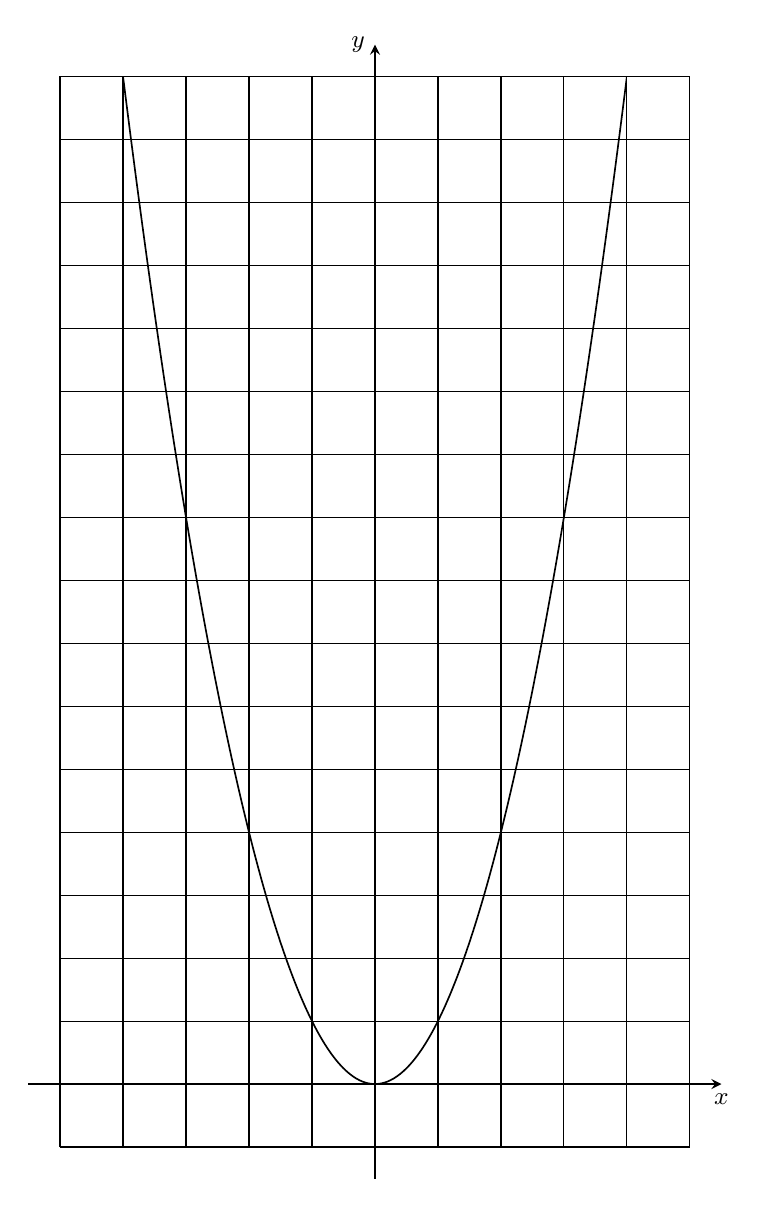
\begin{tikzpicture}[scale=0.8]
    \draw (-5, -1) grid (5, 16);
    \draw[line width=0.6pt, ->, >=stealth] (-5.5, 0) -- (5.5, 0) node[below]{{\small$x$}};
    \draw[line width=0.6pt, ->, >=stealth] (0, -1.5) -- (0, 16.5) node[left]{{\small$y$}};
    \begin{scope}
      \clip (-4.000, -0.050) rectangle (4.000, 16.000);
      \draw[line width=0.6pt] plot[smooth] coordinates
      {
        ( -4.000,  16.000)	        ( -3.900,  15.210)
        ( -3.800,  14.440)	        ( -3.700,  13.690)
        ( -3.600,  12.960)	        ( -3.500,  12.250)
        ( -3.400,  11.560)	        ( -3.300,  10.890)
        ( -3.200,  10.240)	        ( -3.100,   9.610)
        ( -3.000,   9.000)	        ( -2.900,   8.410)
        ( -2.800,   7.840)	        ( -2.700,   7.290)
        ( -2.600,   6.760)	        ( -2.500,   6.250)
        ( -2.400,   5.760)	        ( -2.300,   5.290)
        ( -2.200,   4.840)	        ( -2.100,   4.410)
        ( -2.000,   4.000)	        ( -1.900,   3.610)
        ( -1.800,   3.240)	        ( -1.700,   2.890)
        ( -1.600,   2.560)	        ( -1.500,   2.250)
        ( -1.400,   1.960)	        ( -1.300,   1.690)
        ( -1.200,   1.440)	        ( -1.100,   1.210)
        ( -1.000,   1.000)	        ( -0.900,   0.810)
        ( -0.800,   0.640)	        ( -0.700,   0.490)
        ( -0.600,   0.360)	        ( -0.500,   0.250)
        ( -0.400,   0.160)	        ( -0.300,   0.090)
        ( -0.200,   0.040)	        ( -0.100,   0.010)
        (  0.000,   0.000)	        (  0.100,   0.010)
        (  0.200,   0.040)	        (  0.300,   0.090)
        (  0.400,   0.160)	        (  0.500,   0.250)
        (  0.600,   0.360)	        (  0.700,   0.490)
        (  0.800,   0.640)	        (  0.900,   0.810)
        (  1.000,   1.000)	        (  1.100,   1.210)
        (  1.200,   1.440)	        (  1.300,   1.690)
        (  1.400,   1.960)	        (  1.500,   2.250)
        (  1.600,   2.560)	        (  1.700,   2.890)
        (  1.800,   3.240)	        (  1.900,   3.610)
        (  2.000,   4.000)	        (  2.100,   4.410)
        (  2.200,   4.840)	        (  2.300,   5.290)
        (  2.400,   5.760)	        (  2.500,   6.250)
        (  2.600,   6.760)	        (  2.700,   7.290)
        (  2.800,   7.840)	        (  2.900,   8.410)
        (  3.000,   9.000)	        (  3.100,   9.610)
        (  3.200,  10.240)	        (  3.300,  10.890)
        (  3.400,  11.560)	        (  3.500,  12.250)
        (  3.600,  12.960)	        (  3.700,  13.690)
        (  3.800,  14.440)	        (  3.900,  15.210)
        (  4.000,  16.000)
      };
    \end{scope}
  \end{tikzpicture}
\end{center}

% ------------------------------------------------------------------------------
\end{document}
% ------------------------------------------------------------------------------
